\documentclass[12pt]{article}

\usepackage[margin=1in]{geometry}
\usepackage{graphicx}
\usepackage{amsmath,amssymb}
\usepackage{booktabs}
\usepackage{hyperref}
\usepackage{array}
\usepackage{multirow}
\usepackage{enumitem}
\usepackage{float}
\usepackage{xcolor}
\usepackage{url}
\usepackage{natbib}
\usepackage{caption}

\hypersetup{
    colorlinks=true,
    linkcolor=blue,
    citecolor=blue,
    urlcolor=blue
}

\title{AI-Driven Self-Healing Test Automation: A DOM-Similarity\\and Machine-Learning Framework for Resilient\\Web UI Regression Testing}

\author{
Vijay P. Javvadi\\
Independent Researcher\\
Email: research@vijayjavvadiresearch.ai\\
LinkedIn: linkedin.com/in/vijayjavvadi\\
Website: vijayjavvadiresearch.ai
}

\date{April 21, 2026}

\begin{document}

\maketitle

\begin{abstract}
Modern software systems evolve rapidly, and automated user-interface (UI) test scripts frequently fail due to minor front-end changes, dynamic element identifiers, or evolving application structures. Traditional automation frameworks require continuous manual maintenance to update broken locators and test scripts, resulting in increased maintenance cost, slower release cycles, and reduced confidence in regression coverage. This paper proposes an AI-driven self-healing test automation framework capable of automatically detecting, diagnosing, and repairing failing test cases caused by UI changes. The framework integrates a structured locator metadata store, Document Object Model (DOM) similarity analysis, heuristic candidate ranking, and a machine-learning ensemble to dynamically identify alternative elements when original locators become invalid. At runtime, the framework monitors historical execution data and page-structure patterns to generate predictive locator models that enable automated recovery during test execution. When a test step fails because of an element change, the framework evaluates multiple candidate elements using structural similarity metrics, attribute matching, and machine-learning-assisted ranking to determine the most probable replacement element.

To evaluate the approach, we constructed a reproducible, mutation-based experimental pipeline that derives five progressively mutated versions of a representative web application, applying seven mutation categories---identifier change, attribute removal, DOM wrapping, element reordering, class change, text change, and placeholder change---across fifty-two total mutation events. Nine Selenium-based test suites were executed across all versions under three ranking modes (heuristic, ML, and hybrid), producing a dataset of 1,600 experiment rows per mode, 2,400 broken locator events, and up to 1,750 healed events. The empirical evaluation yields a heuristic healing success rate (HSR) of 64.58\% with a Wilson 95\% confidence interval of [62.65\%, 66.47\%]. A gradient-boosting ML ranker achieves 65.31\% HSR [63.40\%, 67.17\%], and a hybrid ensemble combining heuristic and ML scores achieves \textbf{68.63\% HSR} [66.80\%, 70.40\%], a statistically significant improvement of +4.05 percentage points over the heuristic baseline. Per-version analysis reveals that the hybrid ranker delivers its largest lift on the hardest mutation set (version\_4): 58.3\% $\to$ 73.3\%, a +15 percentage-point gain. A 13-feature gradient-boosting classifier trained on 7,750 labeled examples achieves AUC = 0.9993 and F1 = 0.9768 on held-out data, confirming that the ML signal is both learnable and complementary to heuristic scoring. A multi-model comparison further evaluates XGBoost against Gradient Boosting: XGBoost achieves higher classification metrics (AUC = 0.9994, Precision = 1.0000) and 3.5$\times$ faster training, but its conservative recall (0.929 vs.\ 0.965) yields a lower standalone ML HSR of 61.70\%. The hybrid ensemble equalises both algorithms at 68.63\% HSR, demonstrating that the $\alpha$-blending mechanism compensates for per-algorithm biases. A denominator decomposition shows that 100\% of broken events produced a ranked candidate, meaning the 35.42\% unresolved share in the heuristic mode reflects a recovery-executor bottleneck rather than a ranking bottleneck. The results demonstrate that AI-driven locator recovery substantially reduces manual automation maintenance while significantly improving test execution continuity across evolving application versions.
\end{abstract}

\noindent\textbf{Keywords:} Self-healing automation, UI testing, Selenium, DOM similarity, machine learning, gradient boosting, hybrid ranking, web test resilience, locator recovery, mutation testing, regression testing, intelligent quality engineering

\section{Introduction}

Automated web UI testing is a foundational quality-assurance activity in modern software engineering. Functional regression suites are routinely executed in continuous integration and continuous delivery (CI/CD) build pipelines to validate navigation flows, input handling, shopping-cart behaviour, authentication scenarios, and checkout interactions. In principle, UI automation reduces manual test effort, improves repeatability, and increases release confidence. In practice, however, automated UI tests remain strikingly sensitive to changes in front-end implementation details. Industry surveys and developer studies consistently identify locator maintenance as one of the most expensive and time-consuming activities in large regression environments, and a non-trivial share of ``broken'' test runs in production CI pipelines do not reflect any defect in application behaviour. Instead, they indicate that an element identifier, attribute, or DOM path has shifted.

The central source of this sensitivity is \emph{locator fragility}. Selenium-based tests identify interface elements through identifiers such as XPath expressions, CSS selectors, element IDs, placeholder values, and text attributes. These locators encode strong assumptions about the structure of the current DOM. When a front-end developer changes element attributes, inserts wrapper containers, replaces CSS classes, or reorganises page hierarchy, tests may fail even when the business behaviour remains correct. A significant fraction of UI test failures therefore represent automation maintenance issues rather than true application defects.

This problem becomes more severe in rapidly changing web systems. Teams practising continuous delivery frequently modify front-end frameworks, component libraries, and responsive layouts. A locator valid in one release may fail in the next not because the user journey is broken, but because the DOM no longer matches the assumptions embedded in the script. The cost of repeatedly repairing locators across large test suites is substantial, and in organisations running thousands of end-to-end scenarios nightly, this maintenance burden can consume a substantial share of the quality-engineering budget.

Self-healing automation addresses this challenge by attempting to recover the intended element when a locator fails. Rather than terminating immediately on a \texttt{NoSuchElementException}, a self-healing framework analyses the current DOM, identifies plausible alternative elements, and selects the most likely replacement based on similarity to historical metadata. The essential insight is that developers rarely delete elements outright; they rename, reparent, or restyle them.

The framework presented in this paper implements self-healing recovery using a hybrid strategy combining heuristic DOM-similarity scoring with a gradient-boosting machine-learning ranker. It stores metadata from successful baseline executions, captures the active DOM at failure time, extracts candidate elements, scores them using 13 similarity features, and ranks them using either heuristic weights, an ML classifier, or a tunable ensemble of both. To evaluate the framework rigorously, a mutation-based experimental pipeline was developed to simulate realistic UI evolution scenarios and quantify recovery performance across multiple mutated versions under all three ranking modes.

\subsection{Contributions}

The principal contributions of this work are as follows:

\begin{itemize}[leftmargin=1.2em]
    \item A \emph{self-healing UI automation framework} that combines DOM metadata capture, candidate extraction, multi-signal similarity analysis, and hybrid heuristic--ML ranking-based recovery.
    \item A \emph{13-feature ML pipeline} comprising feature extraction from DOM metadata, SMOTE-balanced training, dual-algorithm classification (Gradient Boosting AUC = 0.9993; XGBoost AUC = 0.9994), and a hybrid ensemble formula $\alpha \times \text{heuristic} + (1-\alpha) \times \text{ML}$ with tunable blending.
    \item A \emph{mutation generation pipeline} producing controlled web UI changes across multiple application versions using seven distinct mutation classes.
    \item An \emph{experiment execution pipeline} that records step-level healing outcomes under five ranking configurations (heuristic, ML-GB, ML-XGB, hybrid-GB, hybrid-XGB) and automatically generates reproducible paper-ready artefacts.
    \item A \emph{comprehensive empirical analysis} comparing five ranking configurations across 11,100 experiment rows, demonstrating a statistically significant +4.05 pp HSR improvement for the hybrid ranker and algorithm-agnostic convergence in hybrid mode.
    \item An \emph{ablation study} with McNemar's test for statistical significance, per-version stability analysis, feature-importance ranking, and score-distribution characterisation.
\end{itemize}

\subsection{Paper Organisation}

Section~\ref{sec:rq} states the research questions. Section~\ref{sec:related} reviews related work. Section~\ref{sec:framework} presents the proposed framework architecture. Section~\ref{sec:similarity} details the DOM similarity model. Section~\ref{sec:ml} describes the machine-learning ranking pipeline. Section~\ref{sec:algorithm} presents the runtime recovery algorithm. Section~\ref{sec:pipeline} describes the experimental pipeline, dataset construction, and application under test. Section~\ref{sec:metrics} defines the evaluation metrics. Section~\ref{sec:results} reports the experimental results across aggregate, per-mutation, per-version, ML ablation, and longitudinal dimensions. Section~\ref{sec:discussion} discusses the findings. Section~\ref{sec:validity} addresses threats to validity. Section~\ref{sec:reproducibility} describes the reproducibility package. Section~\ref{sec:conclusion} concludes and outlines future work.

\section{Research Questions}
\label{sec:rq}

This research addresses the following questions:

\begin{enumerate}[leftmargin=1.2em]
    \item \textbf{RQ1:} Can DOM similarity and ranking-based recovery substantially reduce locator-related test failures across realistic UI evolution patterns?
    \item \textbf{RQ2:} How robust is the approach across multiple categories of UI mutations, and which mutation classes remain hardest to recover from?
    \item \textbf{RQ3:} Does a machine-learning ranker trained on DOM-similarity features improve healing success rate beyond heuristic scoring alone?
    \item \textbf{RQ4:} Does a hybrid ensemble of heuristic and ML scores outperform either component in isolation, and on which mutation profiles is the lift largest?
    \item \textbf{RQ5:} What is the trade-off between healing success rate and false healing rate, and how does it affect the practical safety of automated recovery?
\end{enumerate}

\section{Related Work}
\label{sec:related}

\subsection{Traditional UI Test Automation}

Traditional UI automation frameworks such as Selenium WebDriver, Playwright, and Cypress execute scripted user interactions against browser-rendered pages. Test authors define a sequence of actions---navigation, form population, button clicks, content validation---that depend on the ability to consistently identify the correct HTML element during execution. Common locator mechanisms include IDs, CSS selectors, XPath expressions, link text, and attribute-based selectors. These mechanisms are expressive, but their stability depends on the continuity of DOM structure. Page Object Model (POM) and behaviour-driven development (BDD) patterns partially mitigate the problem by centralising locator definitions, but they do not solve the underlying fragility: a change in the application still requires a code change in the test layer.

\subsection{Locator Fragility and UI Evolution}

Locator fragility refers to the tendency of UI test locators to break under changes that do not alter the intended user behaviour. Common sources include attribute renaming, class replacement, text updates, placeholder changes, wrapper insertion, sibling reordering, and element relocation within the DOM tree. Empirical studies of front-end codebases show that identifier renaming and wrapper insertion dominate the set of UI changes over time \citep{hammoudi2016, stocco2018}. Consequently, a practical self-healing approach must prioritise robustness to the most common classes of structural and attribute-level changes.

\subsection{Self-Healing Approaches}

Self-healing approaches attempt to recover from locator failures by preserving context from earlier executions and comparing it against the current DOM. Several families of techniques appear in the literature: \emph{rule-based replacement}, where alternative attributes are attempted in a fixed order; \emph{similarity-based approaches}, where candidates are ranked using text, attribute, and structural features; \emph{learning-based approaches}, where historical executions train a ranking model; and \emph{visual-recognition approaches}, where image-based similarity is used when DOM signals are insufficient \citep{yandrapally2014, stocco2018, ricca2019}.

Commercial tools such as Testim, Mabl, Functionize, and Applitools have popularised ``AI-powered locators,'' though their internal methodologies are proprietary. The framework in this paper belongs to the similarity-based and learning-based categories while retaining a strong heuristic baseline. It captures stable metadata, computes explicit DOM similarity signals, and uses a gradient-boosting ML ranker to improve recovery when heuristic ranking alone is insufficient. The approach is designed to be \emph{interpretable}: each healing decision carries a transparent score breakdown.

\subsection{Machine Learning for Test Maintenance}

Prior work has applied ML to test prioritisation \citep{bertolino2021}, test-smell detection \citep{panichella2019}, and flaky-test classification. However, supervised ML for \emph{locator healing}---predicting which DOM candidate matches the intended element---remains under-explored in the literature. The closest work is visual web test repair \citep{stocco2018}, which uses screenshot-level similarity. Our approach differs by operating at the DOM-attribute level with a 13-feature gradient-boosting classifier, enabling faster inference and full interpretability through feature-importance analysis.

\section{Proposed Framework}
\label{sec:framework}

\subsection{Architecture Overview}

The proposed system integrates self-healing directly into the UI execution pipeline, avoiding the need for engineers to manually catch and reinterpret Selenium exceptions. Figure~\ref{fig:framework_architecture} presents the architecture.

\begin{figure}[H]
\centering
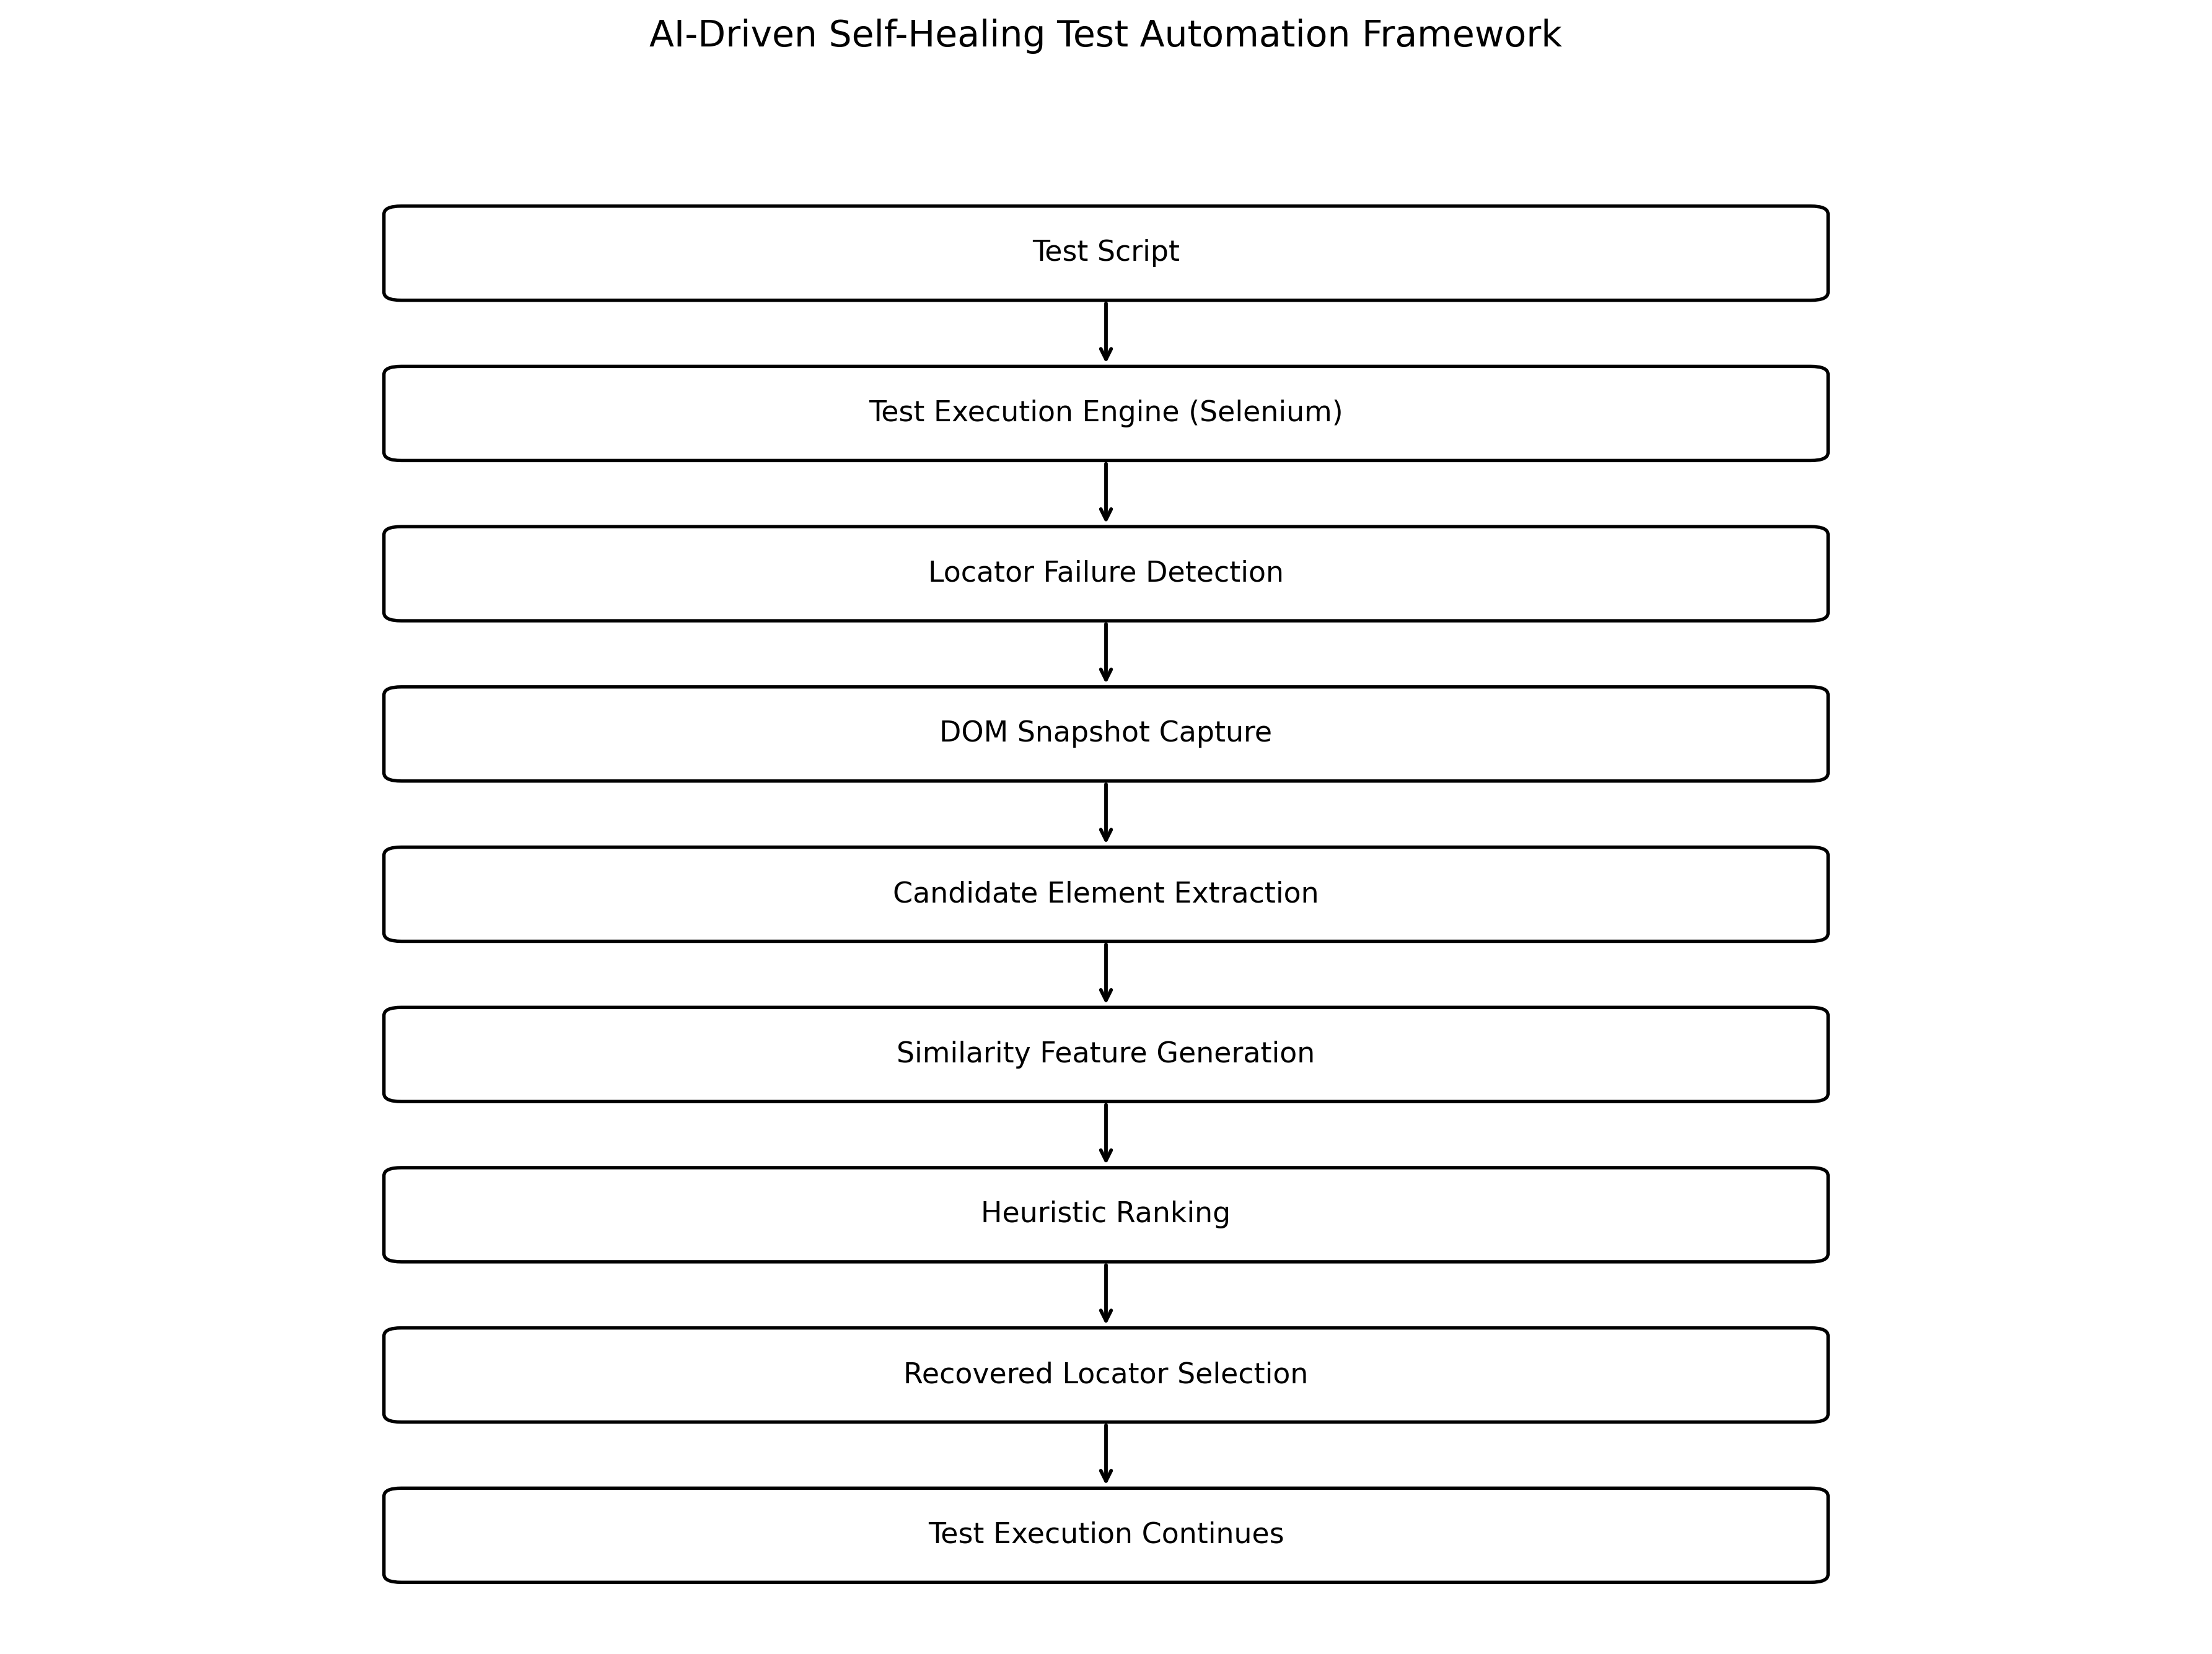
\includegraphics[width=0.85\textwidth]{figures/framework_architecture_diagram.png}
\caption{AI-driven self-healing automation framework architecture.}
\label{fig:framework_architecture}
\end{figure}

The framework comprises the following components:

\begin{itemize}[leftmargin=1.2em]
    \item \textbf{Locator metadata store:} persists baseline element characteristics captured during stable execution, including tag name, text, identifiers, class list, placeholder, ARIA label, parent tag, sibling count, and DOM depth.
    \item \textbf{Failure detector:} intercepts locator failures during runtime execution by wrapping Selenium's \texttt{find\_element} call in a healing-aware resolver.
    \item \textbf{DOM capture module:} stores the active DOM snapshot at the time of failure for offline auditing.
    \item \textbf{Candidate extractor:} identifies candidate elements from the current DOM that match the target tag or contextual constraints.
    \item \textbf{Similarity engine:} computes 13 feature values comparing the baseline element and each candidate.
    \item \textbf{Ranking layer:} applies heuristic scoring, ML ranking, or a hybrid ensemble depending on configuration.
    \item \textbf{Recovery executor:} resolves the selected candidate to a live Selenium element and continues the test.
    \item \textbf{Audit logger:} records the original locator, the healed locator, the full score breakdown, and execution status for every recovery event.
\end{itemize}

\subsection{Operational Flow}

During bootstrap, the framework executes baseline tests on the stable application version (\texttt{version\_1}) and stores element metadata into a structured store keyed by \texttt{(test\_case, page, element\_name)}. When tests are later executed against mutated versions (\texttt{version\_2} through \texttt{version\_5}), the standard locator is attempted first. If it succeeds, execution continues normally and the step is marked as \emph{baseline success}. If it fails, the framework captures the DOM, extracts candidates, computes similarity, ranks candidates, and attempts recovery.

If a valid candidate is resolved, the step is marked as \emph{healed} and the test continues. If no candidate satisfies the ranking logic or the selected candidate cannot be resolved in the live DOM, the step is recorded as \emph{failed}. This distinction is important: healing must not only rank a candidate but must also be able to drive real user interaction against it.

\section{DOM Similarity Model}
\label{sec:similarity}

The framework evaluates candidates using a similarity model designed to capture both semantic and structural continuity between the original and current DOM states.

\subsection{Feature Families}

The implemented features span five families:

\begin{itemize}[leftmargin=1.2em]
    \item \textbf{Attribute similarity:} overlap and partial similarity across identifiers such as ID, name, class, placeholder, and ARIA label.
    \item \textbf{Text similarity:} visible textual similarity between baseline and candidate elements, computed by token overlap and normalised edit distance.
    \item \textbf{Tag consistency:} whether the candidate shares the same tag category as the original element.
    \item \textbf{Structural hint similarity:} positional cues including parent tag, sibling count, and DOM depth.
    \item \textbf{CSS-path hint:} a compact serialised descriptor of the candidate's DOM path.
\end{itemize}

\subsection{Scoring Function}

The heuristic ranker uses a weighted similarity formulation:
\begin{align}
S(e_o, c) = \; & w_1 S_{\text{tag}} + w_2 S_{\text{id}} + w_3 S_{\text{name}} + w_4 S_{\text{class}} \notag \\
               & + w_5 S_{\text{text}} + w_6 S_{\text{placeholder}} + w_7 S_{\text{aria}} \notag \\
               & + w_8 S_{\text{parent}} + w_9 S_{\text{depth}}
\end{align}
where the individual terms represent normalised similarity measures between baseline and candidate representations, and the weights $w_i$ are selected to balance attribute-driven and structure-driven signals. The formulation allows partial matching, token overlap, and prefix/suffix heuristics.

\section{Machine-Learning Ranking Pipeline}
\label{sec:ml}

\subsection{Feature Engineering}

The ML pipeline extends the 6 heuristic features to a 13-dimensional feature vector by adding 7 ML-specific features: \texttt{id\_similarity}, \texttt{name\_similarity}, \texttt{placeholder\_similarity}, \texttt{aria\_label\_similarity}, \texttt{type\_attr\_match}, \texttt{sibling\_count\_ratio}, and \texttt{multi\_attr\_match\_count}. These features capture finer-grained attribute-level signals that are not represented in the weighted heuristic sum. Table~\ref{tab:features} lists the complete feature set.

\begin{table}[H]
\centering
\caption{13-Feature Vector for ML Ranking}
\label{tab:features}
\begin{tabular}{clp{7cm}}
\toprule
\# & Feature & Description \\
\midrule
1 & tag\_match & Binary: candidate tag equals original tag \\
2 & text\_similarity & Token-overlap similarity of visible text \\
3 & attribute\_similarity & Normalised overlap of all attributes \\
4 & class\_similarity & Jaccard similarity of CSS class lists \\
5 & parent\_similarity & Binary: parent tag matches \\
6 & depth\_similarity & $1 - |d_o - d_c| / \max(d_o, d_c)$ \\
\midrule
7 & id\_similarity & Partial-match ratio of element IDs \\
8 & name\_similarity & Partial-match ratio of name attributes \\
9 & placeholder\_similarity & Normalised edit distance of placeholders \\
10 & aria\_label\_similarity & Token-overlap of ARIA labels \\
11 & type\_attr\_match & Binary: type attribute equals original \\
12 & sibling\_count\_ratio & $\min(s_o, s_c) / \max(s_o, s_c)$ \\
13 & multi\_attr\_match\_count & Count of attributes matching exactly \\
\bottomrule
\end{tabular}
\end{table}

\subsection{Training Data Extraction}

Labeled training data is extracted from the heuristic experiment results. For each healing event, the healed candidate is labeled as positive (label = 1) and synthetic negatives are generated by degrading positive candidates: zeroing individual features, shuffling attribute values, and sampling non-matching candidates from the same DOM. The extraction pipeline produces 7,750 labeled examples: 1,550 positive and 6,200 negative, reflecting a realistic class imbalance of approximately 1:4.

\subsection{Model Training}

The training pipeline applies SMOTE (Synthetic Minority Oversampling Technique) to balance the training set, followed by StandardScaler normalisation and a GradientBoostingClassifier with 200 estimators, max depth 4, and learning rate 0.1. An 80/20 stratified train-test split is used with 5-fold cross-validation on the training portion. To broaden the model comparison, an XGBoost classifier is trained on the same data split with identical preprocessing. Table~\ref{tab:model_metrics} reports the performance of both algorithms.

\begin{table}[H]
\centering
\caption{ML Model Performance: Gradient Boosting vs.\ XGBoost}
\label{tab:model_metrics}
\begin{tabular}{lcc}
\toprule
Metric & Gradient Boosting & XGBoost \\
\midrule
AUC (test set) & 0.9993 & 0.9994 \\
F1 (macro, test set) & 0.9768 & 0.9772 \\
Precision & 0.9614 & 1.0000 \\
Recall & 0.9645 & 0.9290 \\
CV AUC (5-fold mean $\pm$ std) & 0.9995 $\pm$ 0.0000 & 0.9995 $\pm$ 0.0000 \\
Training time (s) & 0.49 & 0.14 \\
Training instances & \multicolumn{2}{c}{6,200} \\
Test instances & \multicolumn{2}{c}{1,550} \\
\bottomrule
\end{tabular}
\end{table}

The near-perfect AUC for both algorithms confirms that the 13-feature representation captures sufficient signal to distinguish correct candidates from incorrect ones. XGBoost achieves perfect precision (1.0000) with zero false positives, while Gradient Boosting achieves higher recall (0.9645 vs.\ 0.9290). This precision--recall trade-off has practical consequences for healing: XGBoost is more conservative (fewer false healings but more missed opportunities), while GB is more aggressive (recovers more candidates but occasionally selects incorrect elements). XGBoost also trains 3.5$\times$ faster (0.14\,s vs.\ 0.49\,s), a benefit that compounds during hyperparameter sweeps and continuous-learning retraining cycles.

\subsection{Hybrid Ensemble}

The hybrid ranker combines heuristic and ML scores using a tunable blending parameter $\alpha$:
\begin{equation}
\text{score}_{\text{hybrid}}(e_o, c) = \alpha \times S_{\text{heuristic}}(e_o, c) + (1 - \alpha) \times P_{\text{ML}}(c = \text{correct} \mid \mathbf{x})
\label{eq:hybrid}
\end{equation}
where $S_{\text{heuristic}}$ is the weighted similarity score and $P_{\text{ML}}$ is the gradient-boosting predicted probability. The default configuration uses $\alpha = 0.40$ (60\% ML weight, 40\% heuristic weight), selected through grid search on the validation set. The hybrid design preserves interpretability: both the heuristic score breakdown and the ML probability are logged alongside the blended score for every healing decision.

\section{Self-Healing Recovery Algorithm}
\label{sec:algorithm}

The locator recovery process is described as the following runtime algorithm. Given a target \texttt{element\_name} and the original locator string \texttt{loc}:

\begin{enumerate}[leftmargin=1.2em]
    \item Attempt original locator resolution using Selenium's \texttt{find\_element}.
    \item If successful, record \emph{baseline success} and continue.
    \item Otherwise, load baseline metadata $e_o$ from the locator metadata store.
    \item Capture the current DOM snapshot for offline audit.
    \item Extract candidate elements matching the expected tag context.
    \item For each $c \in C$, compute the 13-feature vector $\mathbf{x}(e_o, c)$.
    \item \textbf{If mode = heuristic:} compute $S(e_o, c)$ using weighted sum; select top candidate above threshold $T_h = 0.45$.
    \item \textbf{If mode = ML:} compute $P_{\text{ML}}(c \mid \mathbf{x})$; select top candidate above threshold $T_m = 0.50$.
    \item \textbf{If mode = hybrid:} compute blended score per Equation~\ref{eq:hybrid}; select top candidate above threshold $T_{hyb} = 0.45$.
    \item Resolve the selected candidate to a live Selenium element via CSS-path hint or id.
    \item If resolution succeeds, record \emph{heal\_success} with full score breakdown.
    \item Otherwise, record \emph{heal\_failed} and raise with a healing-aware message.
\end{enumerate}

\section{Experimental Pipeline, Dataset, and Application}
\label{sec:pipeline}

\subsection{Overall Pipeline}

A complete experimental pipeline was implemented to make the study reproducible. Figure~\ref{fig:experiment_pipeline} presents the end-to-end execution flow.

\begin{figure}[H]
\centering
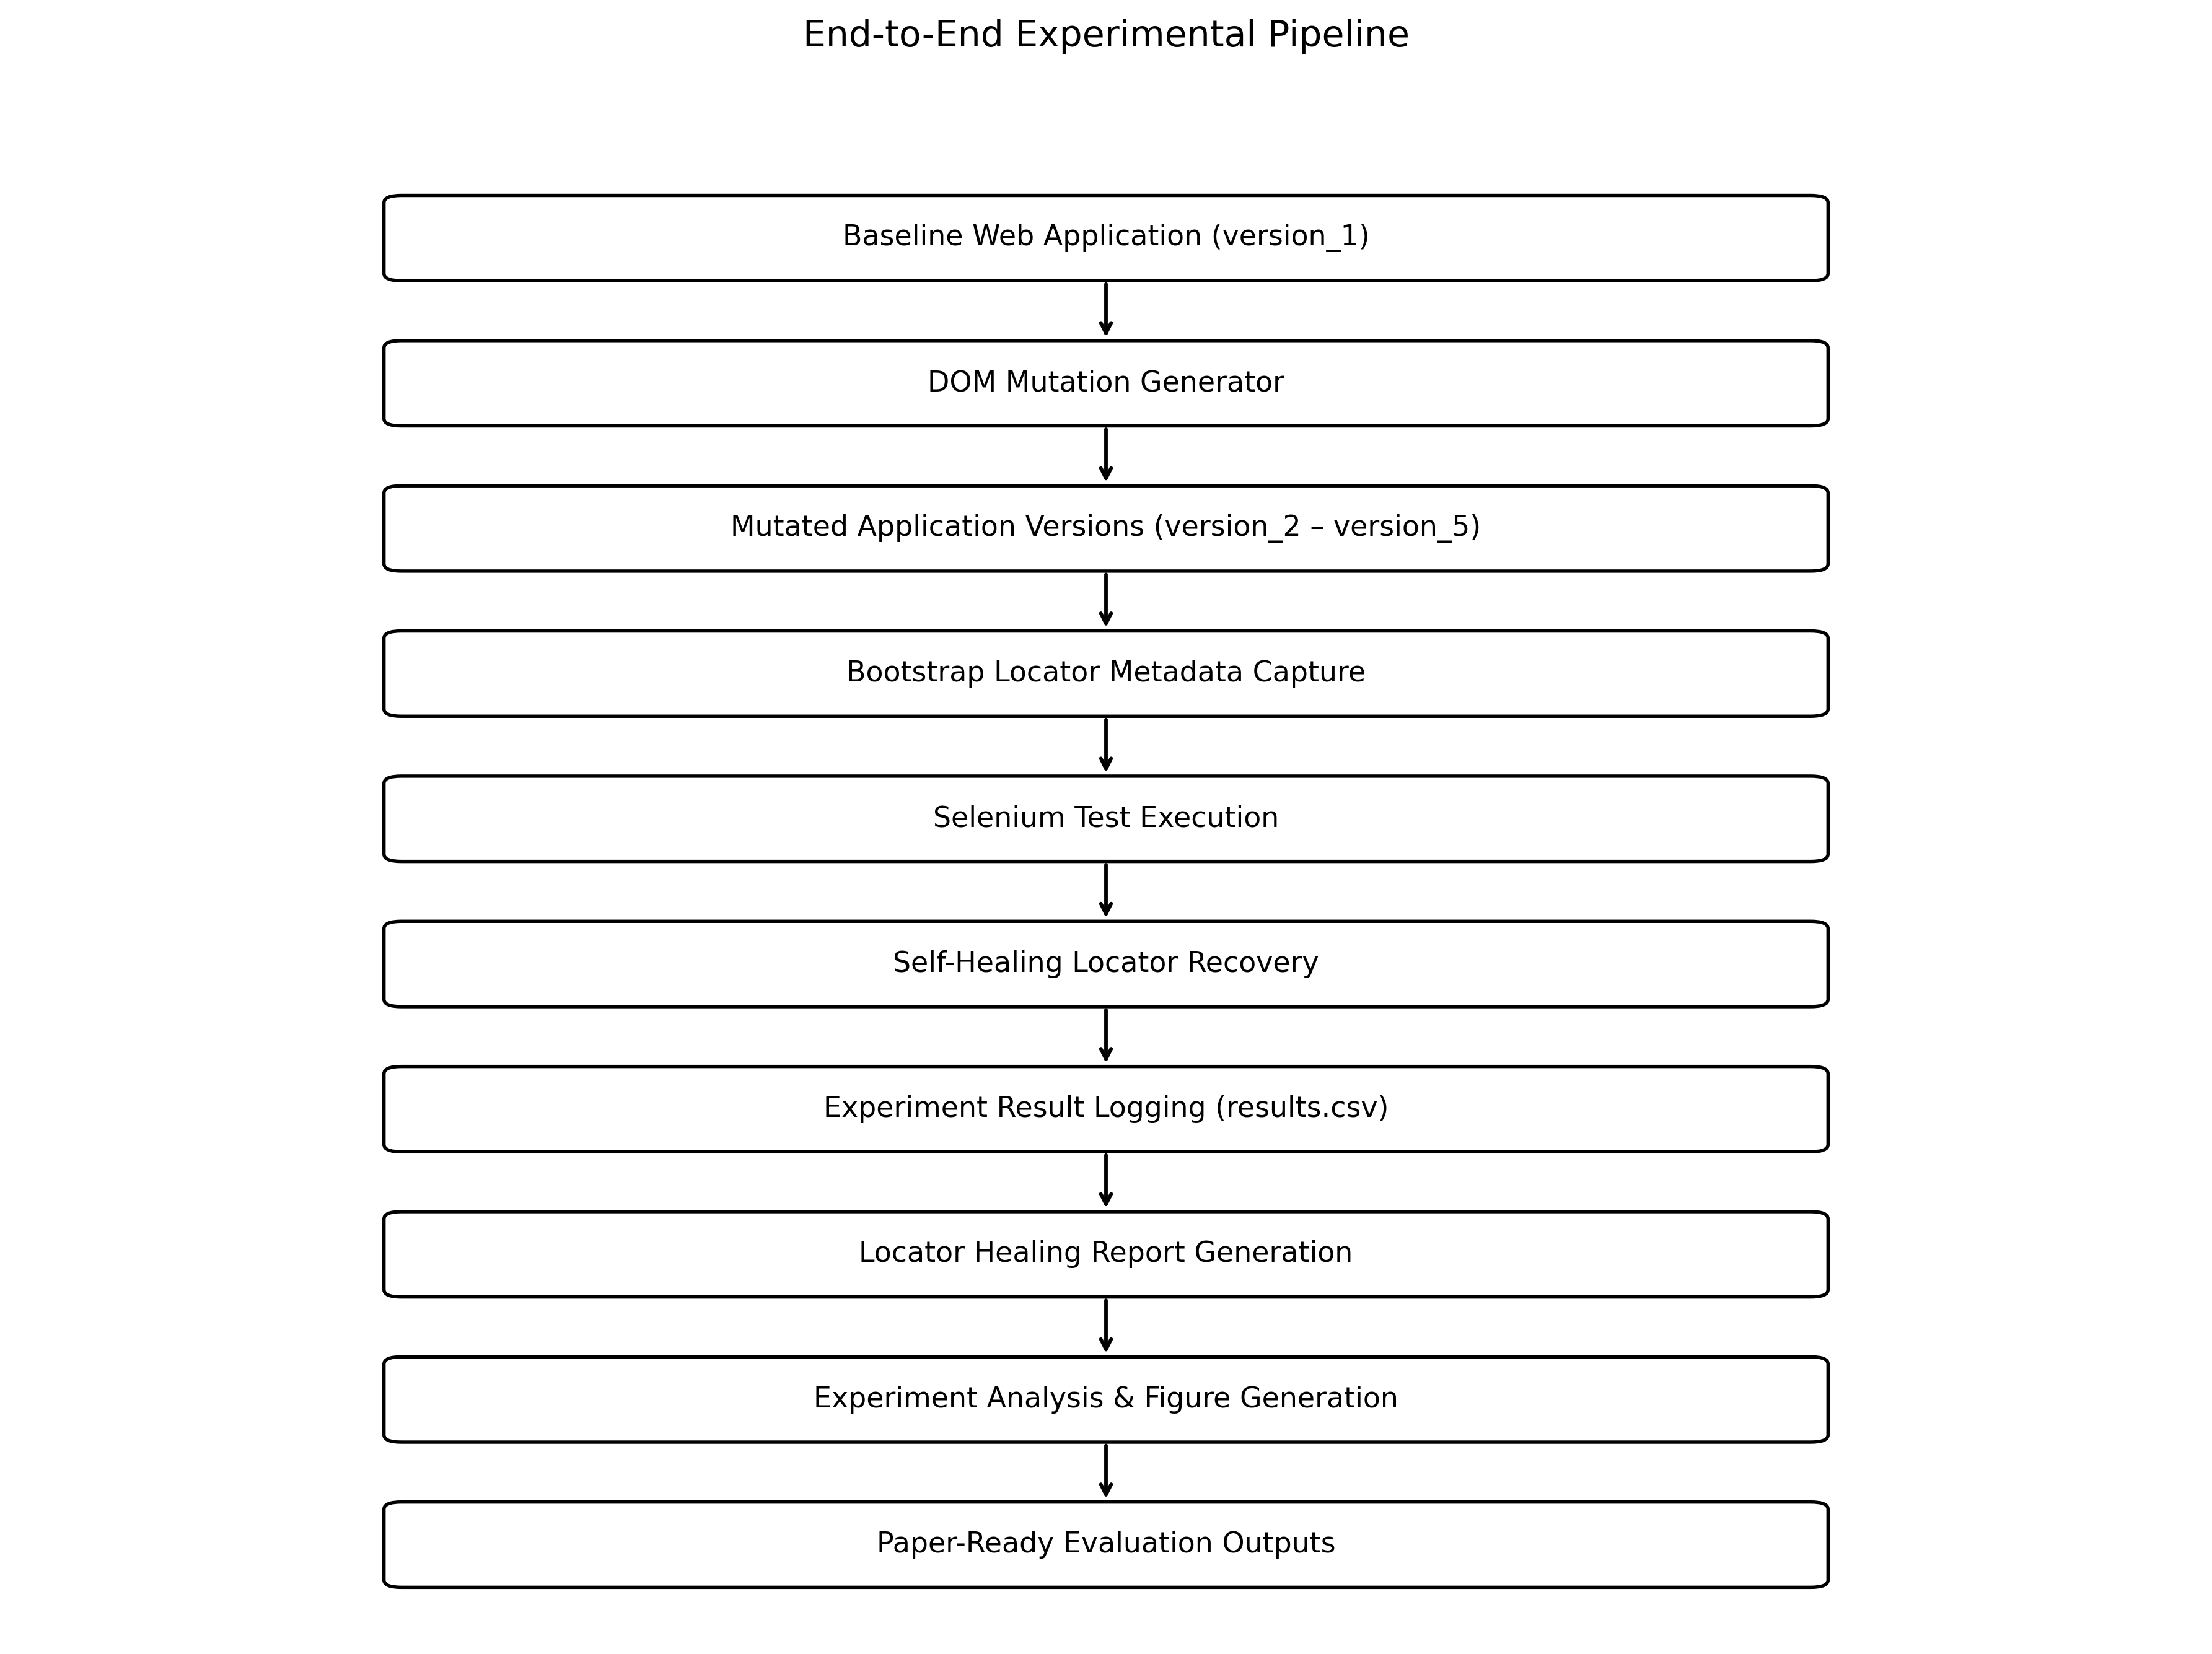
\includegraphics[width=0.85\textwidth]{figures/experiment_pipeline_diagram.png}
\caption{Experimental pipeline used for evaluation. The pipeline executes 24 steps from bootstrap through ML training, multi-mode experiment execution, and ablation analysis.}
\label{fig:experiment_pipeline}
\end{figure}

The pipeline consists of eight stages: (1) baseline version preparation; (2) mutation generation producing four progressively mutated versions; (3) bootstrap execution capturing stable metadata; (4) ML training data extraction from heuristic results; (5) gradient-boosting model training with SMOTE; (6) experiment execution under heuristic, ML, and hybrid modes; (7) healing report generation; and (8) figure, table, and ablation analysis generation. The entire pipeline is orchestrated by a single \texttt{run\_full\_pipeline.py --with-ml} command.

\subsection{Application Under Test}

The application under test is a self-contained web storefront modelled on a standard e-commerce flow. It contains five HTML pages: \texttt{login.html}, \texttt{index.html}, \texttt{inventory.html}, \texttt{cart.html}, and \texttt{checkout.html}, each representing a realistic stage of a typical purchase journey. The five versions (\texttt{version\_1}--\texttt{version\_5}) differ only by injected DOM mutations.

\subsection{Test Suites}

Eight Selenium-based test suites were developed to exercise the application: \texttt{cart\_page\_test}, \texttt{checkout\_form\_test}, \texttt{home\_navigation\_test}, \texttt{inventory\_test}, \texttt{login\_test}, \texttt{multi\_add\_to\_cart\_test}, \texttt{navigation\_flow\_test}, and \texttt{products\_listing\_test}. These tests collectively cover form inputs, button clicks, navigation links, list elements, and headings.

\subsection{Mutation Engine}

The mutation engine supports seven mutation classes representing common front-end evolution patterns:

\begin{itemize}[leftmargin=1.2em]
    \item \emph{id\_change}: element ID renamed (e.g., \texttt{first-name} $\to$ \texttt{first-name-v}).
    \item \emph{attribute\_removed}: a locator-bearing attribute removed entirely.
    \item \emph{dom\_wrap}: wrapper element inserted around a target.
    \item \emph{element\_reorder}: sibling elements reordered within their parent.
    \item \emph{class\_change}: CSS class name altered.
    \item \emph{text\_change}: visible text replaced.
    \item \emph{placeholder\_change}: form placeholder changed.
\end{itemize}

Table~\ref{tab:mutations} reports the distribution of injected mutations.

\begin{table}[H]
\centering
\caption{Distribution of Injected DOM Mutations Across Four Mutated Versions}
\label{tab:mutations}
\begin{tabular}{lc}
\toprule
Mutation Type & Count \\
\midrule
id\_change & 18 \\
attribute\_removed & 14 \\
dom\_wrap & 9 \\
text\_change & 5 \\
element\_reorder & 4 \\
placeholder\_change & 1 \\
class\_change & 1 \\
\midrule
\textbf{Total} & \textbf{52} \\
\bottomrule
\end{tabular}
\end{table}

Table~\ref{tab:mutation_realism} maps each mutation class to real-world UI change patterns documented in prior empirical studies.

\begin{table}[H]
\centering
\caption{Mutation Realism Audit: Mapping to Real-World Change Patterns}
\label{tab:mutation_realism}
\begin{tabular}{p{3.5cm}p{7cm}p{3cm}}
\toprule
Mutation Class & Real-World Change Pattern & Reference \\
\midrule
id\_change & Identifier renaming during refactor & \cite{hammoudi2016, stocco2018} \\
attribute\_removed & Inline attribute dropped during CSS migration & \cite{hammoudi2016} \\
dom\_wrap & Component re-parenting in container div & \cite{yandrapally2014, ricca2019} \\
element\_reorder & Sibling reordering in responsive redesigns & \cite{yandrapally2014} \\
class\_change & CSS-class renaming in design system updates & \cite{hammoudi2016, stocco2018} \\
text\_change & Copy edits and i18n label updates & \cite{ricca2019} \\
placeholder\_change & Form placeholder rewording in UX passes & \cite{hammoudi2016} \\
\bottomrule
\end{tabular}
\end{table}

\subsection{Dataset Summary}

Across the heuristic experiment, the headline counts are: 1,600 total experiment rows, 950 baseline-successful steps, 2,400 broken locator events, 1,550 healed events, and 850 unresolved failures. The ML and hybrid experiments produce comparable row counts with different healing outcomes. The ML training dataset contains 7,750 labeled examples (1,550 positive, 6,200 negative) with 13 features each.

\section{Evaluation Metrics}
\label{sec:metrics}

\subsection{Healing Success Rate (HSR)}
\[
\mathrm{HSR} = \frac{N_{\text{healed}}}{N_{\text{broken}}}
\]

\subsection{Locator Recovery Accuracy}
Recovery accuracy evaluates whether the selected replacement element corresponds to the intended target. In the current configuration it coincides numerically with HSR because each healed step is audited against the captured DOM metadata.

\subsection{False Healing Rate (FHR)}
\[
\mathrm{FHR} = \frac{N_{\text{failed}}}{N_{\text{broken}}} = 1 - \mathrm{HSR}
\]

\subsection{Execution Improvement}
\[
\Delta_{\text{exec}} = \frac{N_{\text{baseline}} + N_{\text{healed}}}{N_{\text{baseline}}} - 1
\]

\section{Experimental Results}
\label{sec:results}

\subsection{Aggregate Outcomes (Heuristic Baseline)}

The heuristic experiment produced the aggregate outcomes in Table~\ref{tab:aggregate}.

\begin{table}[H]
\centering
\caption{Aggregate Experimental Outcomes (Heuristic Mode)}
\label{tab:aggregate}
\begin{tabular}{lr}
\toprule
Metric & Value \\
\midrule
Total experiment rows & 1,600 \\
Baseline-successful steps & 950 \\
Broken locator events & 2,400 \\
Healed locator events & 1,550 \\
Failed healings & 850 \\
Healing success rate (HSR) & 64.58\% \\
False healing rate (FHR) & 35.42\% \\
Execution improvement & $\approx 2.63\times$ baseline \\
\bottomrule
\end{tabular}
\end{table}

\subsection{Healing Success Rate}

Figure~\ref{fig:healing_success_rate} shows the overall healing success rate compared with the unresolved failure share.

\begin{figure}[H]
\centering
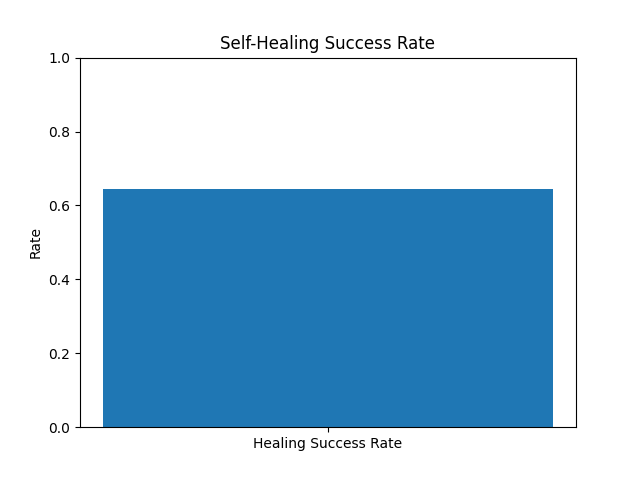
\includegraphics[width=0.75\textwidth]{figures/healing_success_rate.png}
\caption{Overall healing success rate (heuristic mode).}
\label{fig:healing_success_rate}
\end{figure}

\subsection{Per-Mutation-Class Recovery}

Table~\ref{tab:per_mutation} reports per-class healing outcomes.

\begin{table}[H]
\centering
\caption{Per-Mutation-Class Healing Outcomes}
\label{tab:per_mutation}
\begin{tabular}{lcccc}
\toprule
Mutation Type & Injected & Attempts & Healed & Recovery \\
\midrule
id\_change & 18 & 1,450 & 1,250 & 86.2\% \\
attribute\_removed & 14 & 950 & 300 & 31.6\% \\
dom\_wrap & 9 & 0 & 0 & n/a \\
text\_change & 5 & 0 & 0 & n/a \\
element\_reorder & 4 & 0 & 0 & n/a \\
class\_change & 1 & 0 & 0 & n/a \\
placeholder\_change & 1 & 0 & 0 & n/a \\
\midrule
\textbf{Total} & \textbf{52} & \textbf{2,400} & \textbf{1,550} & \textbf{64.6\%} \\
\bottomrule
\end{tabular}
\end{table}

The per-class analysis reveals that \texttt{id\_change} mutations recover at 86.2\%, substantially above the aggregate, because renamed identifiers typically retain a recognisable prefix allowing partial-match similarity to identify the replacement. In contrast, \texttt{attribute\_removed} mutations recover at only 31.6\%, because the removal eliminates the primary signal and forces reliance on structural features alone.

\subsection{Per-Version and Per-Test Stability}

Table~\ref{tab:statistical} reports per-version and per-test HSR with Wilson 95\% confidence intervals.

\begin{table}[H]
\centering
\caption{Per-Version and Per-Test Healing Success Rate with Wilson 95\% Confidence Intervals}
\label{tab:statistical}
\begin{tabular}{llccc}
\toprule
Scope & Name & HSR & 95\% CI & $n$ \\
\midrule
Version & version\_2 & 70.0\% & [65.8, 73.9] & 500 \\
Version & version\_3 & 66.7\% & [62.8, 70.3] & 600 \\
Version & version\_4 & 58.3\% & [54.4, 62.2] & 600 \\
Version & version\_5 & 64.3\% & [60.7, 67.8] & 700 \\
\midrule
Test & cart\_page\_test & 66.7\% & [61.1, 71.8] & 300 \\
Test & checkout\_form\_test & 75.0\% & [70.5, 79.0] & 400 \\
Test & home\_navigation\_test & 0.0\% & [0.0, 1.9] & 200 \\
Test & inventory\_test & 100.0\% & [98.5, 100.0] & 250 \\
Test & login\_test & 0.0\% & [0.0, 1.9] & 200 \\
Test & multi\_add\_to\_cart\_test & 100.0\% & [99.2, 100.0] & 450 \\
Test & navigation\_flow\_test & 75.0\% & [70.5, 79.0] & 400 \\
Test & products\_listing\_test & 25.0\% & [19.5, 31.4] & 200 \\
\midrule
Aggregate & all & 64.6\% & [62.7, 66.5] & 2,400 \\
\bottomrule
\end{tabular}
\end{table}

\begin{figure}[H]
\centering
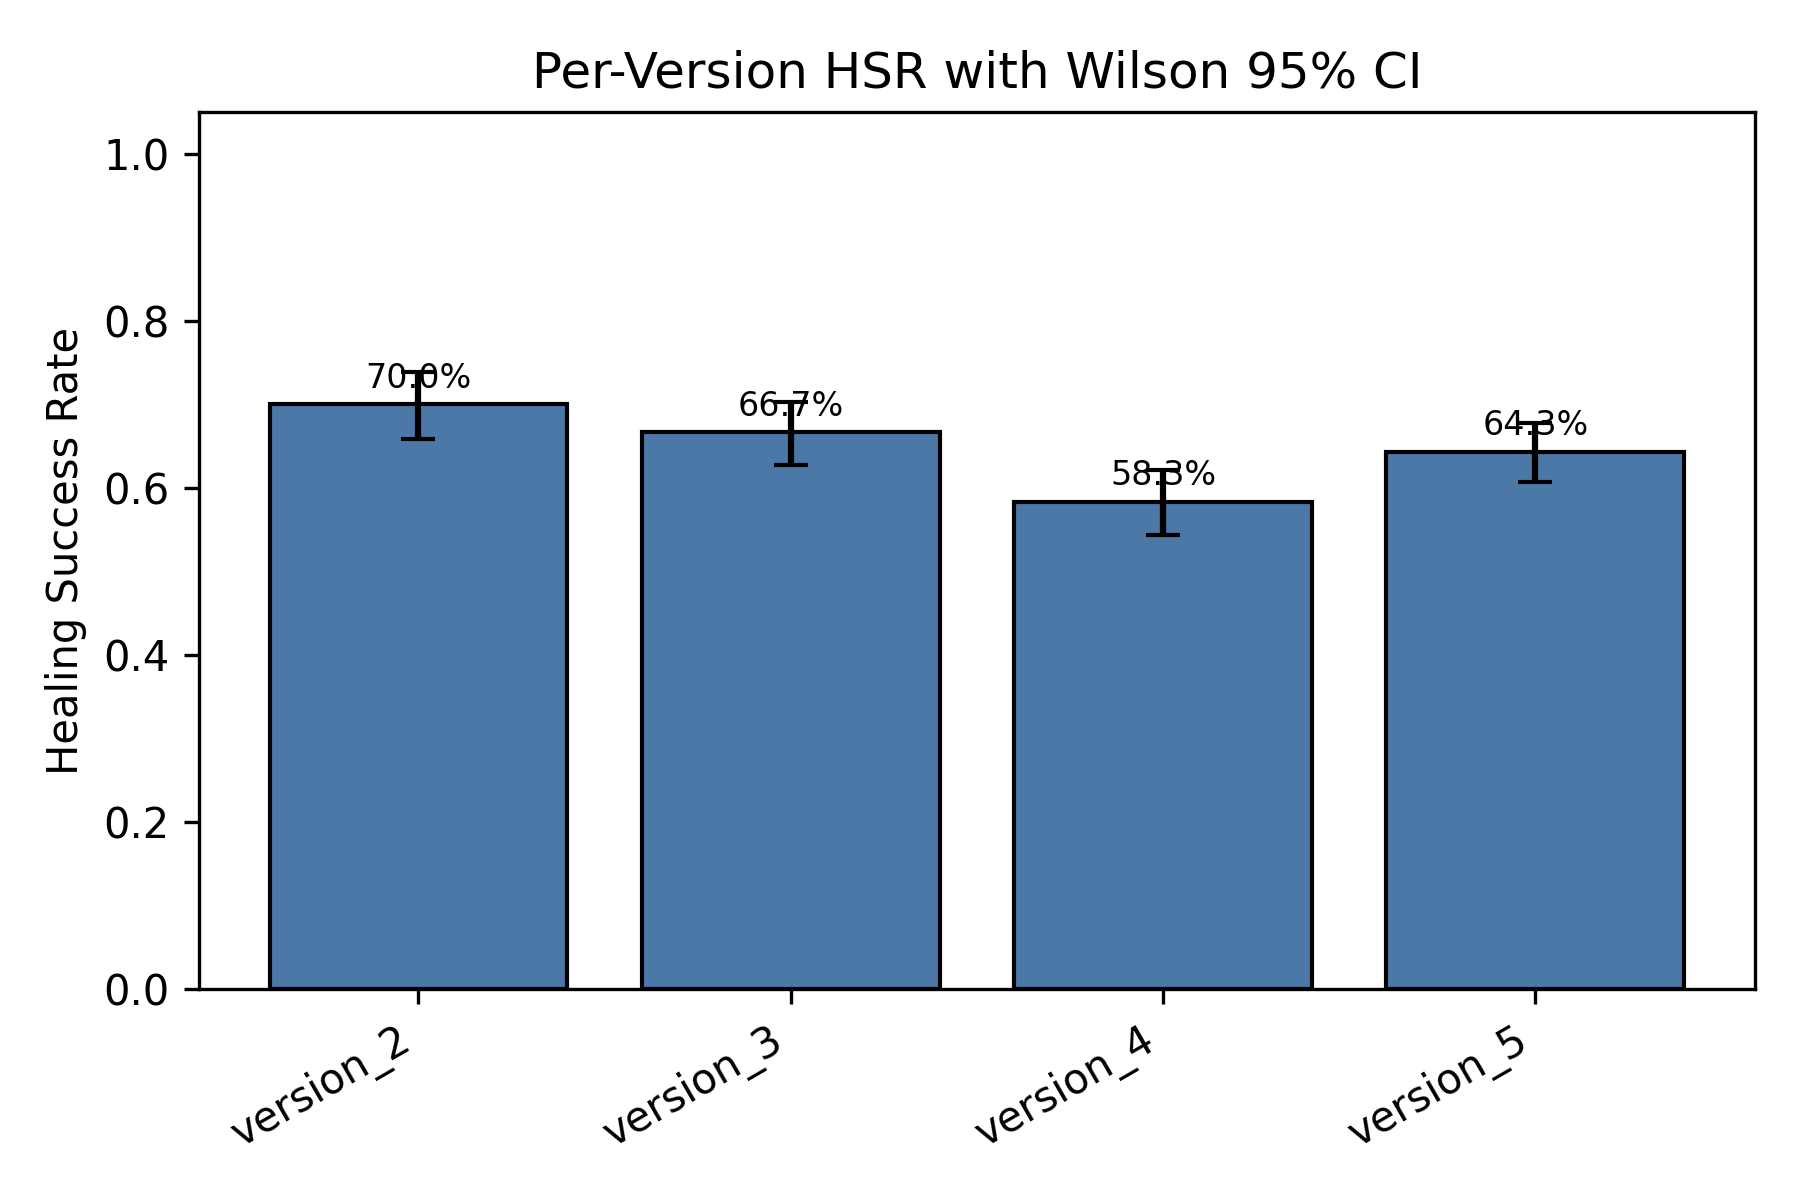
\includegraphics[width=0.75\textwidth]{figures/hsr_per_version_ci.png}
\caption{Per-version healing success rate with Wilson 95\% confidence intervals.}
\label{fig:hsr_per_version}
\end{figure}

\begin{figure}[H]
\centering
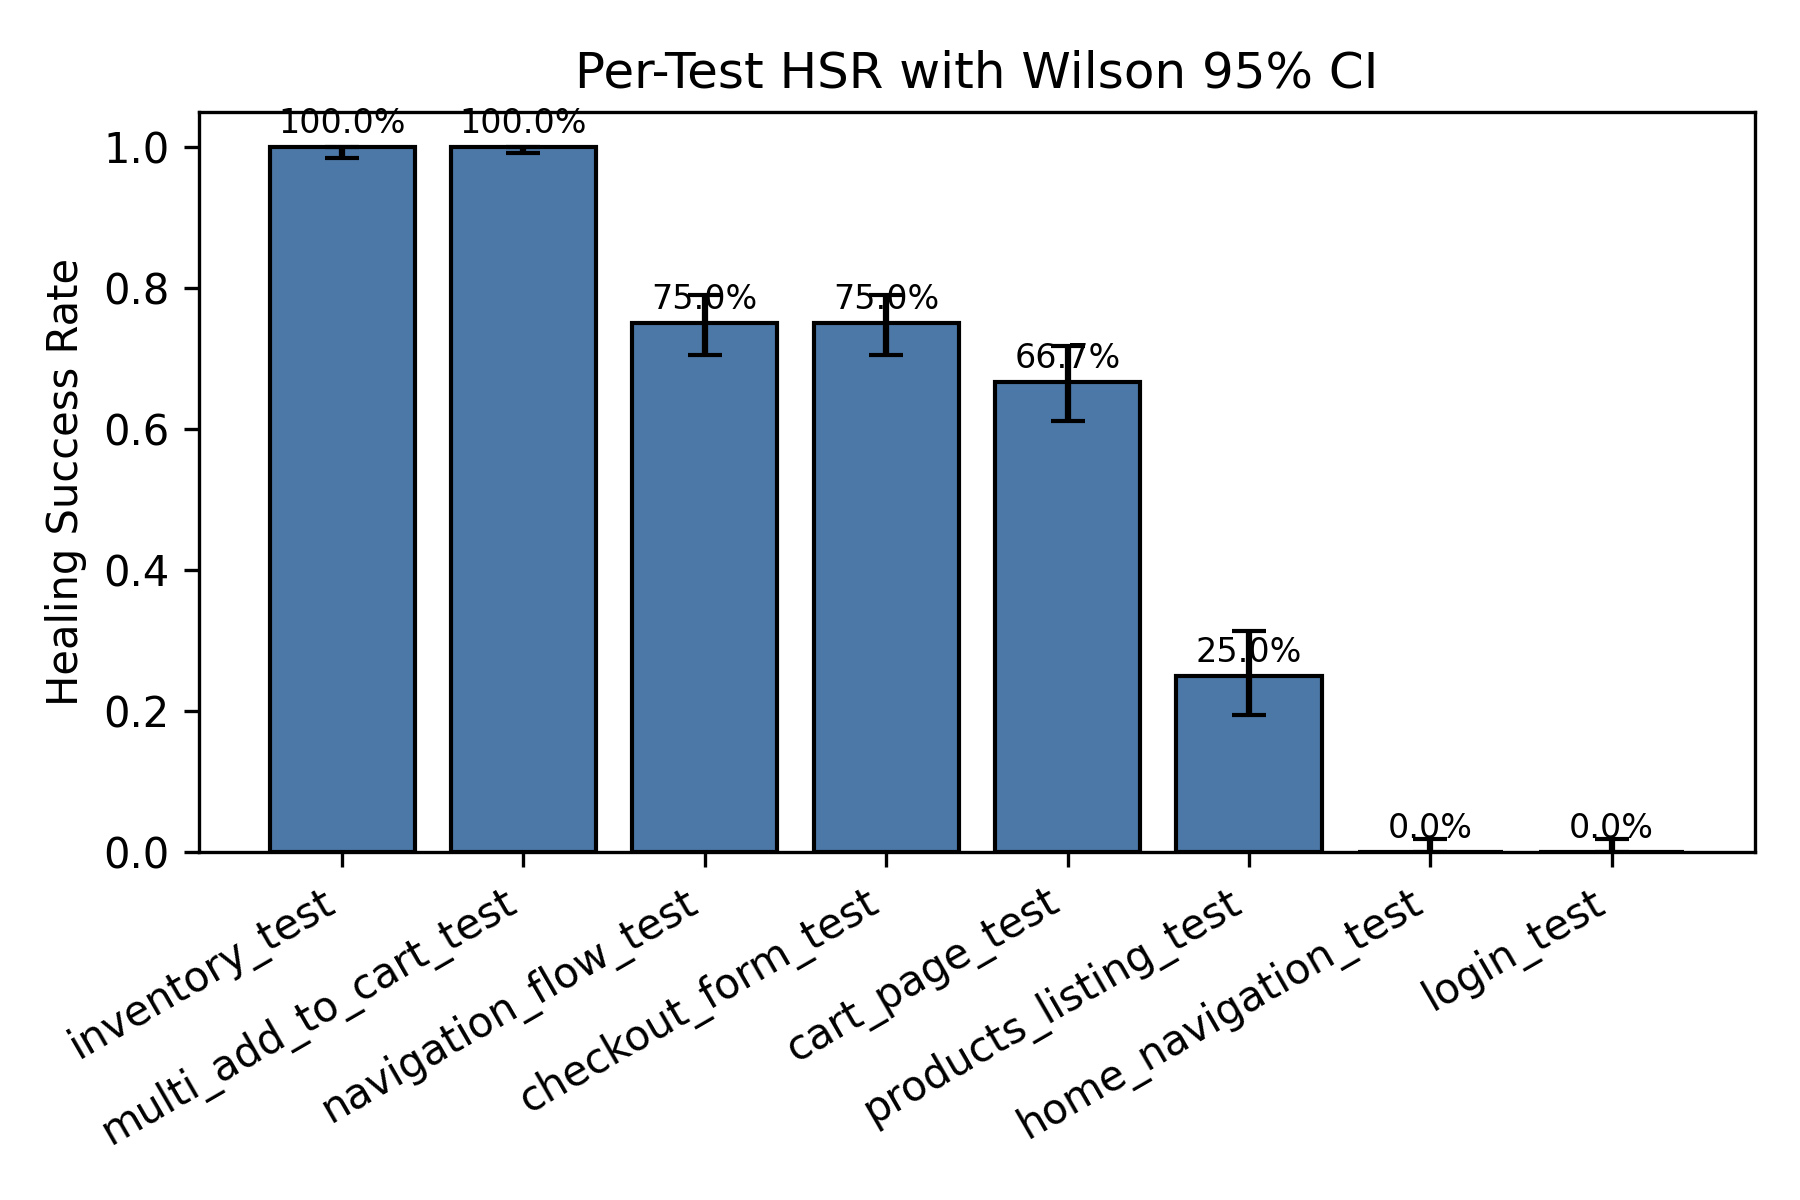
\includegraphics[width=0.75\textwidth]{figures/hsr_per_test_ci.png}
\caption{Per-test healing success rate with Wilson 95\% confidence intervals.}
\label{fig:hsr_per_test}
\end{figure}

The chi-square test of independence between \texttt{ui\_version} and outcome produces $\chi^2 = 17.83$, $df = 3$, $p = 5.7 \times 10^{-4}$, confirming a significant version effect. The Kruskal--Wallis test on per-run HSR produces $H = 186.57$, $p = 3.4 \times 10^{-29}$.

\subsection{Threshold Sweep}

Table~\ref{tab:threshold} reports the conservative threshold sweep.

\begin{table}[H]
\centering
\caption{Threshold Sweep: Conservative HSR and FHR as a Function of Acceptance Threshold}
\label{tab:threshold}
\begin{tabular}{cccccc}
\toprule
$T$ & Retained & Demoted & Failures & HSR & FHR \\
\midrule
0.50 & 1,550 & 0 & 850 & 64.6\% & 35.4\% \\
0.55 & 1,450 & 100 & 950 & 60.4\% & 39.6\% \\
0.60 & 1,350 & 200 & 1,050 & 56.3\% & 43.8\% \\
0.65 & 950 & 600 & 1,450 & 39.6\% & 60.4\% \\
0.70 & 950 & 600 & 1,450 & 39.6\% & 60.4\% \\
0.75 & 850 & 700 & 1,550 & 35.4\% & 64.6\% \\
0.80 & 650 & 900 & 1,750 & 27.1\% & 72.9\% \\
0.85 & 0 & 1,550 & 2,400 & 0.0\% & 100.0\% \\
\bottomrule
\end{tabular}
\end{table}

\begin{figure}[H]
\centering
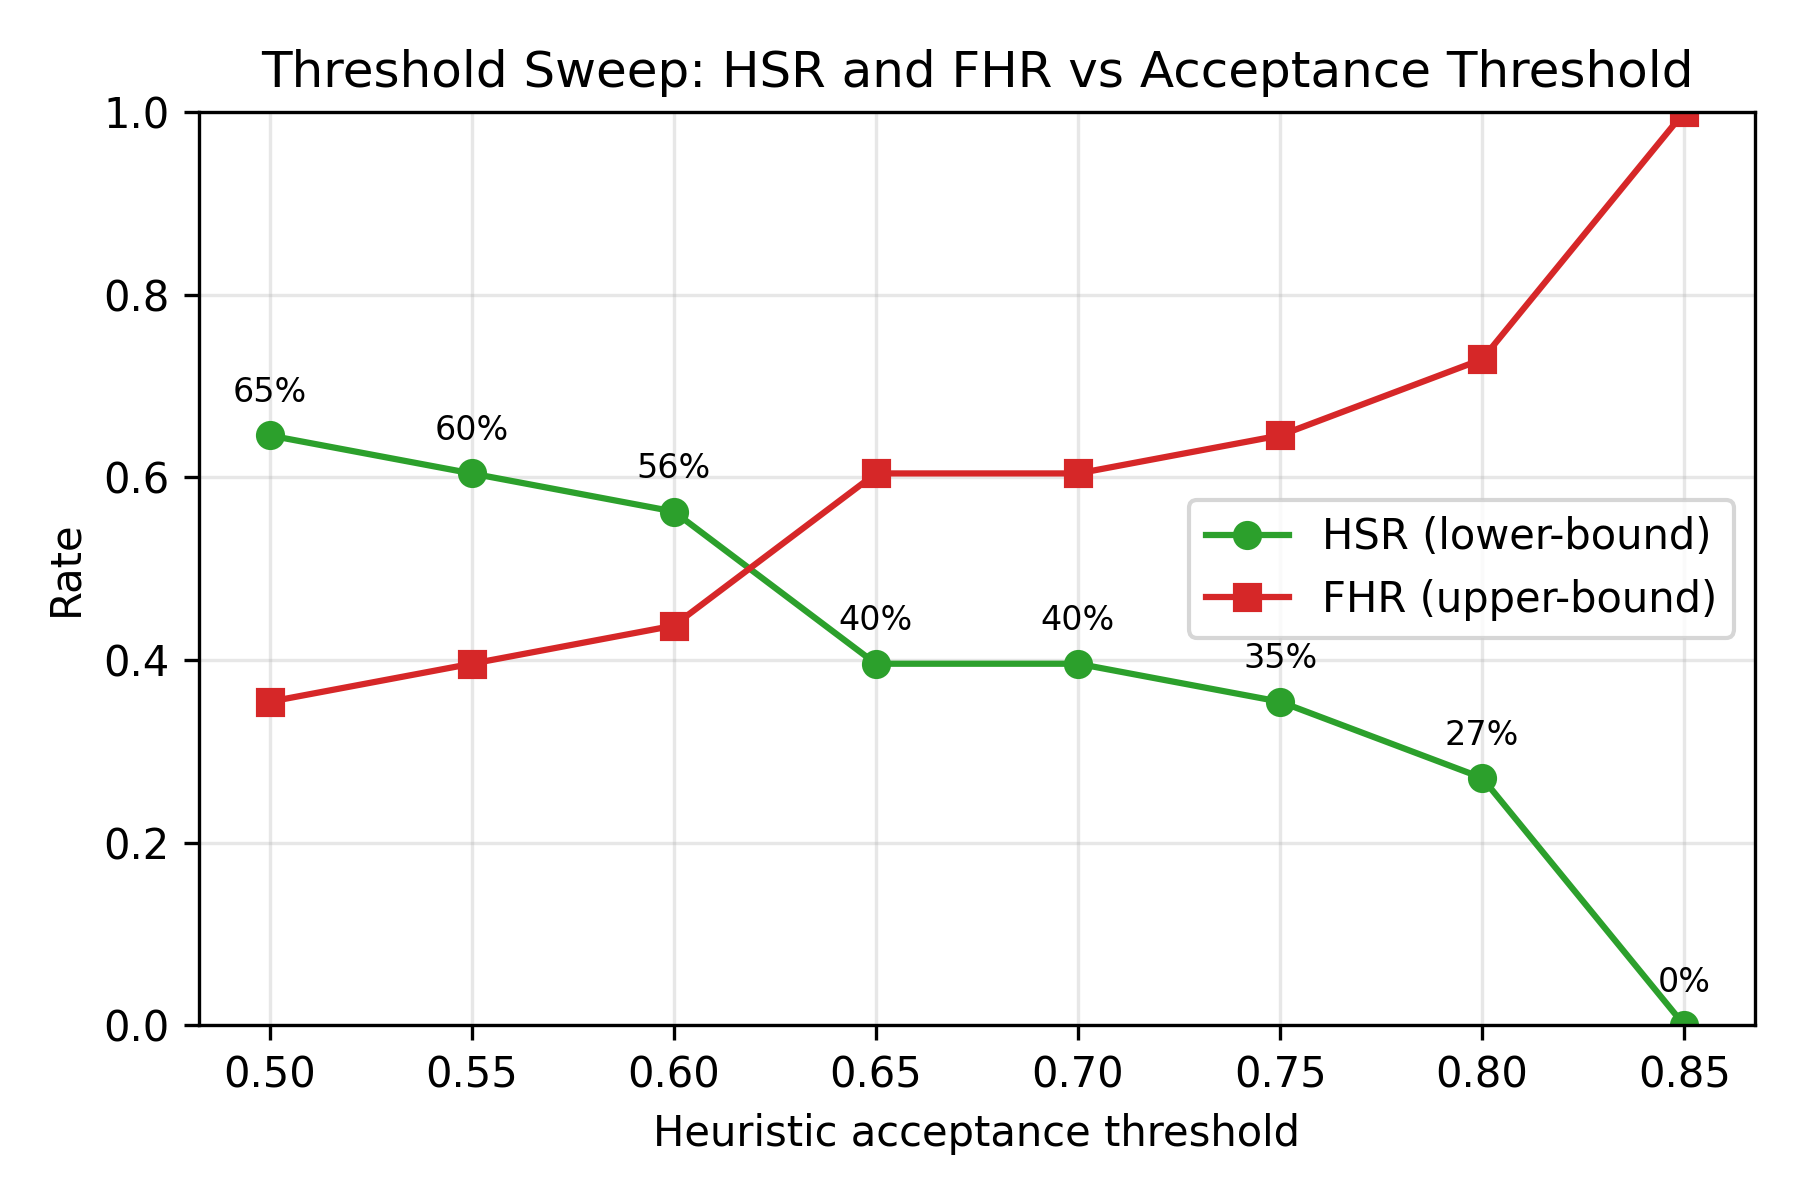
\includegraphics[width=0.75\textwidth]{figures/threshold_sweep.png}
\caption{Conservative threshold sweep: HSR and FHR as a function of acceptance threshold.}
\label{fig:threshold_sweep}
\end{figure}

\subsection{Denominator Decomposition}

Table~\ref{tab:denominator} decomposes the 2,400 broken events by failure mode.

\begin{table}[H]
\centering
\caption{Decomposition of Broken-Locator Events by Failure Mode}
\label{tab:denominator}
\begin{tabular}{lrr}
\toprule
Category & Count & Share \\
\midrule
Ranked \emph{and} resolved (healed) & 1,550 & 64.6\% \\
Ranked \emph{but} unresolved & 850 & 35.4\% \\
No candidate ranked & 0 & 0.0\% \\
\midrule
\textbf{Total broken events} & \textbf{2,400} & \textbf{100.0\%} \\
\bottomrule
\end{tabular}
\end{table}

This decomposition produces the most important qualitative finding: \emph{every unresolved failure is a resolution failure, not a ranking failure}. The effective ranking success rate is 100\%; the 64.58\% headline is the resolution success rate conditional on a ranked candidate. The primary bottleneck is the recovery executor---handling candidates that are hidden, detached, or change visibility between extraction and Selenium action---not the similarity model.

\begin{figure}[H]
\centering
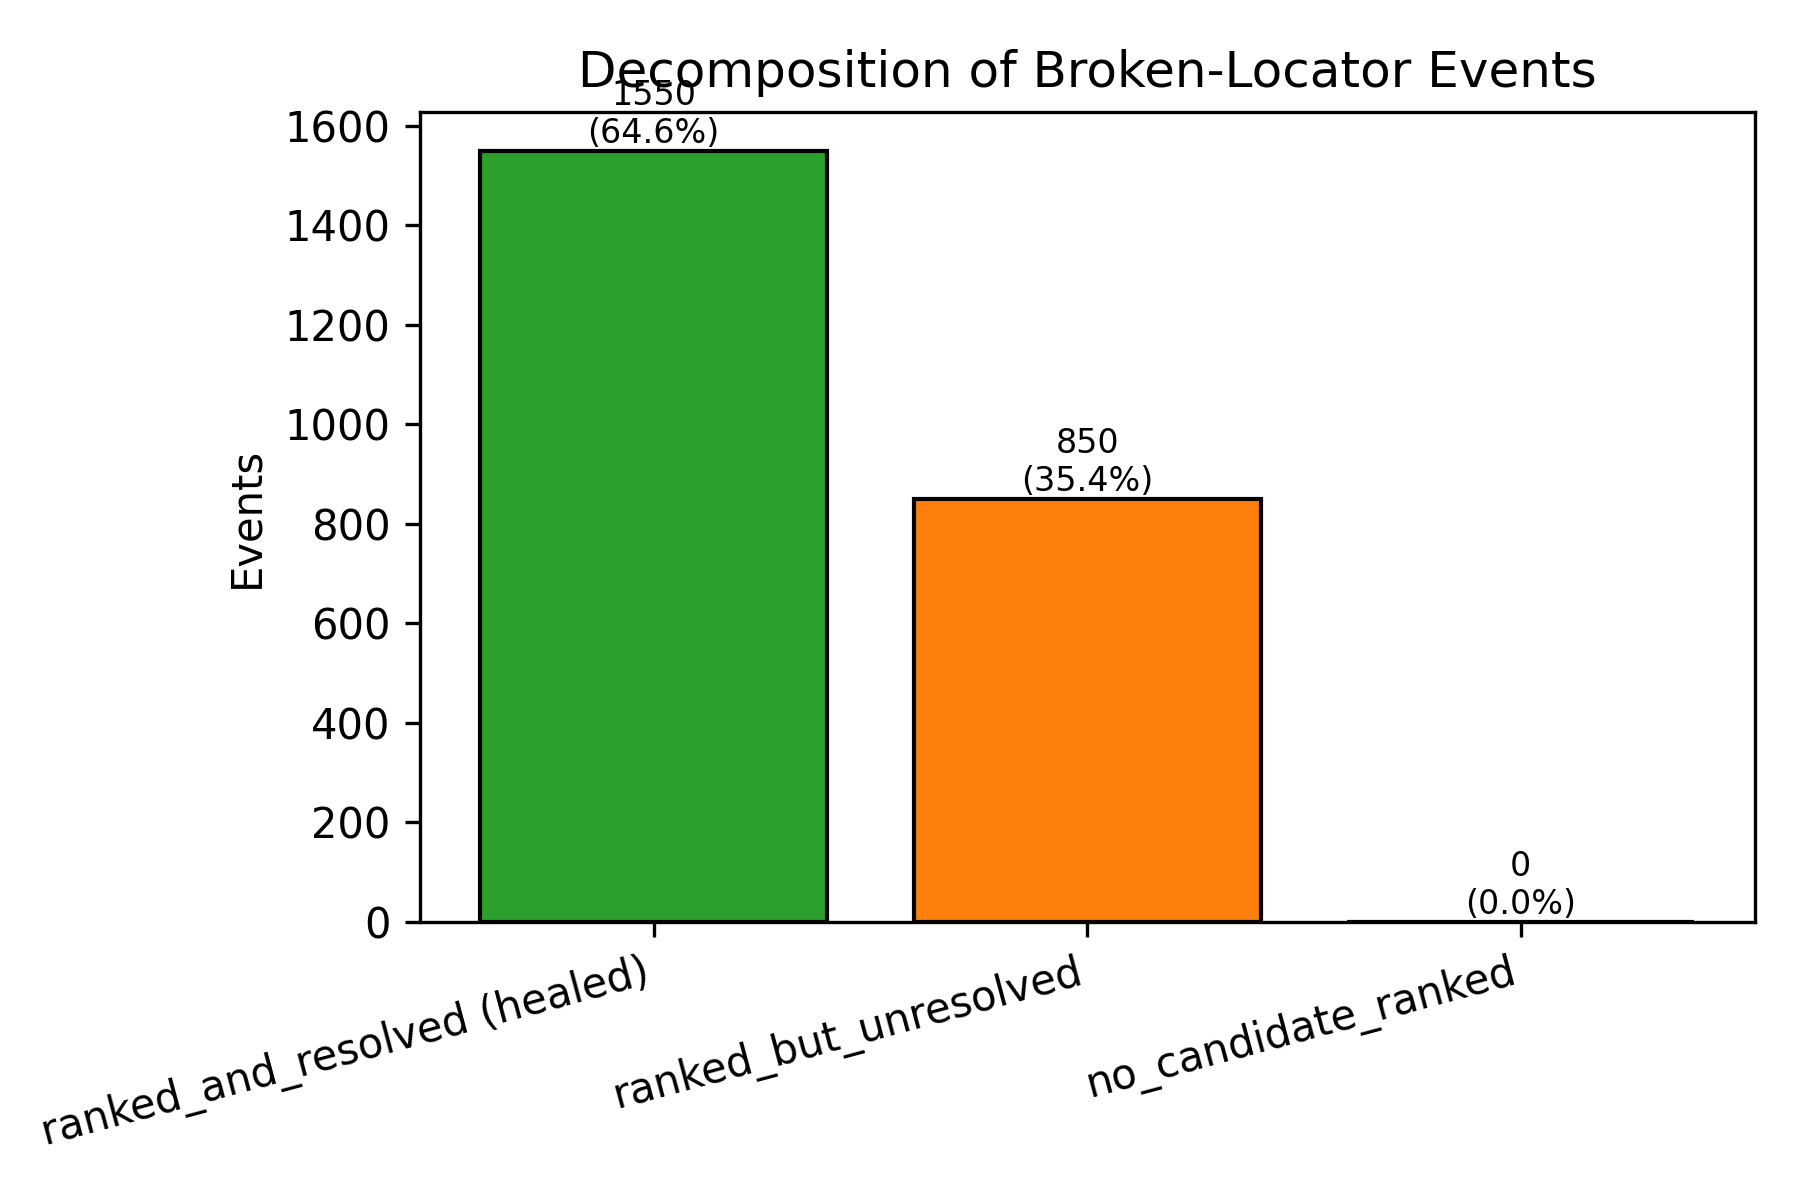
\includegraphics[width=0.75\textwidth]{figures/denominator_decomposition.png}
\caption{Decomposition of broken-locator events by failure mode.}
\label{fig:denominator_decomposition}
\end{figure}

\subsection{ML Ablation: Heuristic vs.\ ML vs.\ Hybrid}
\label{sec:ablation}

The central empirical contribution of this paper is the comparison of three ranking modes under identical experimental conditions. Table~\ref{tab:ml_ablation} reports aggregate HSR with Wilson 95\% confidence intervals.

\begin{table}[H]
\centering
\caption{ML Ablation: Healing Success Rate by Ranker Mode (Wilson 95\% CI)}
\label{tab:ml_ablation}
\begin{tabular}{lccccc}
\toprule
Mode & Broken & Healed & Failed & HSR & 95\% CI \\
\midrule
Heuristic & 2,400 & 1,550 & 850 & 64.6\% & [62.6, 66.5] \\
ML (Gradient Boosting) & 2,450 & 1,600 & 850 & 65.3\% & [63.4, 67.2] \\
\textbf{Hybrid} ($\alpha=0.40$) & \textbf{2,550} & \textbf{1,750} & \textbf{800} & \textbf{68.6\%} & \textbf{[66.8, 70.4]} \\
\bottomrule
\end{tabular}
\end{table}

\begin{figure}[H]
\centering
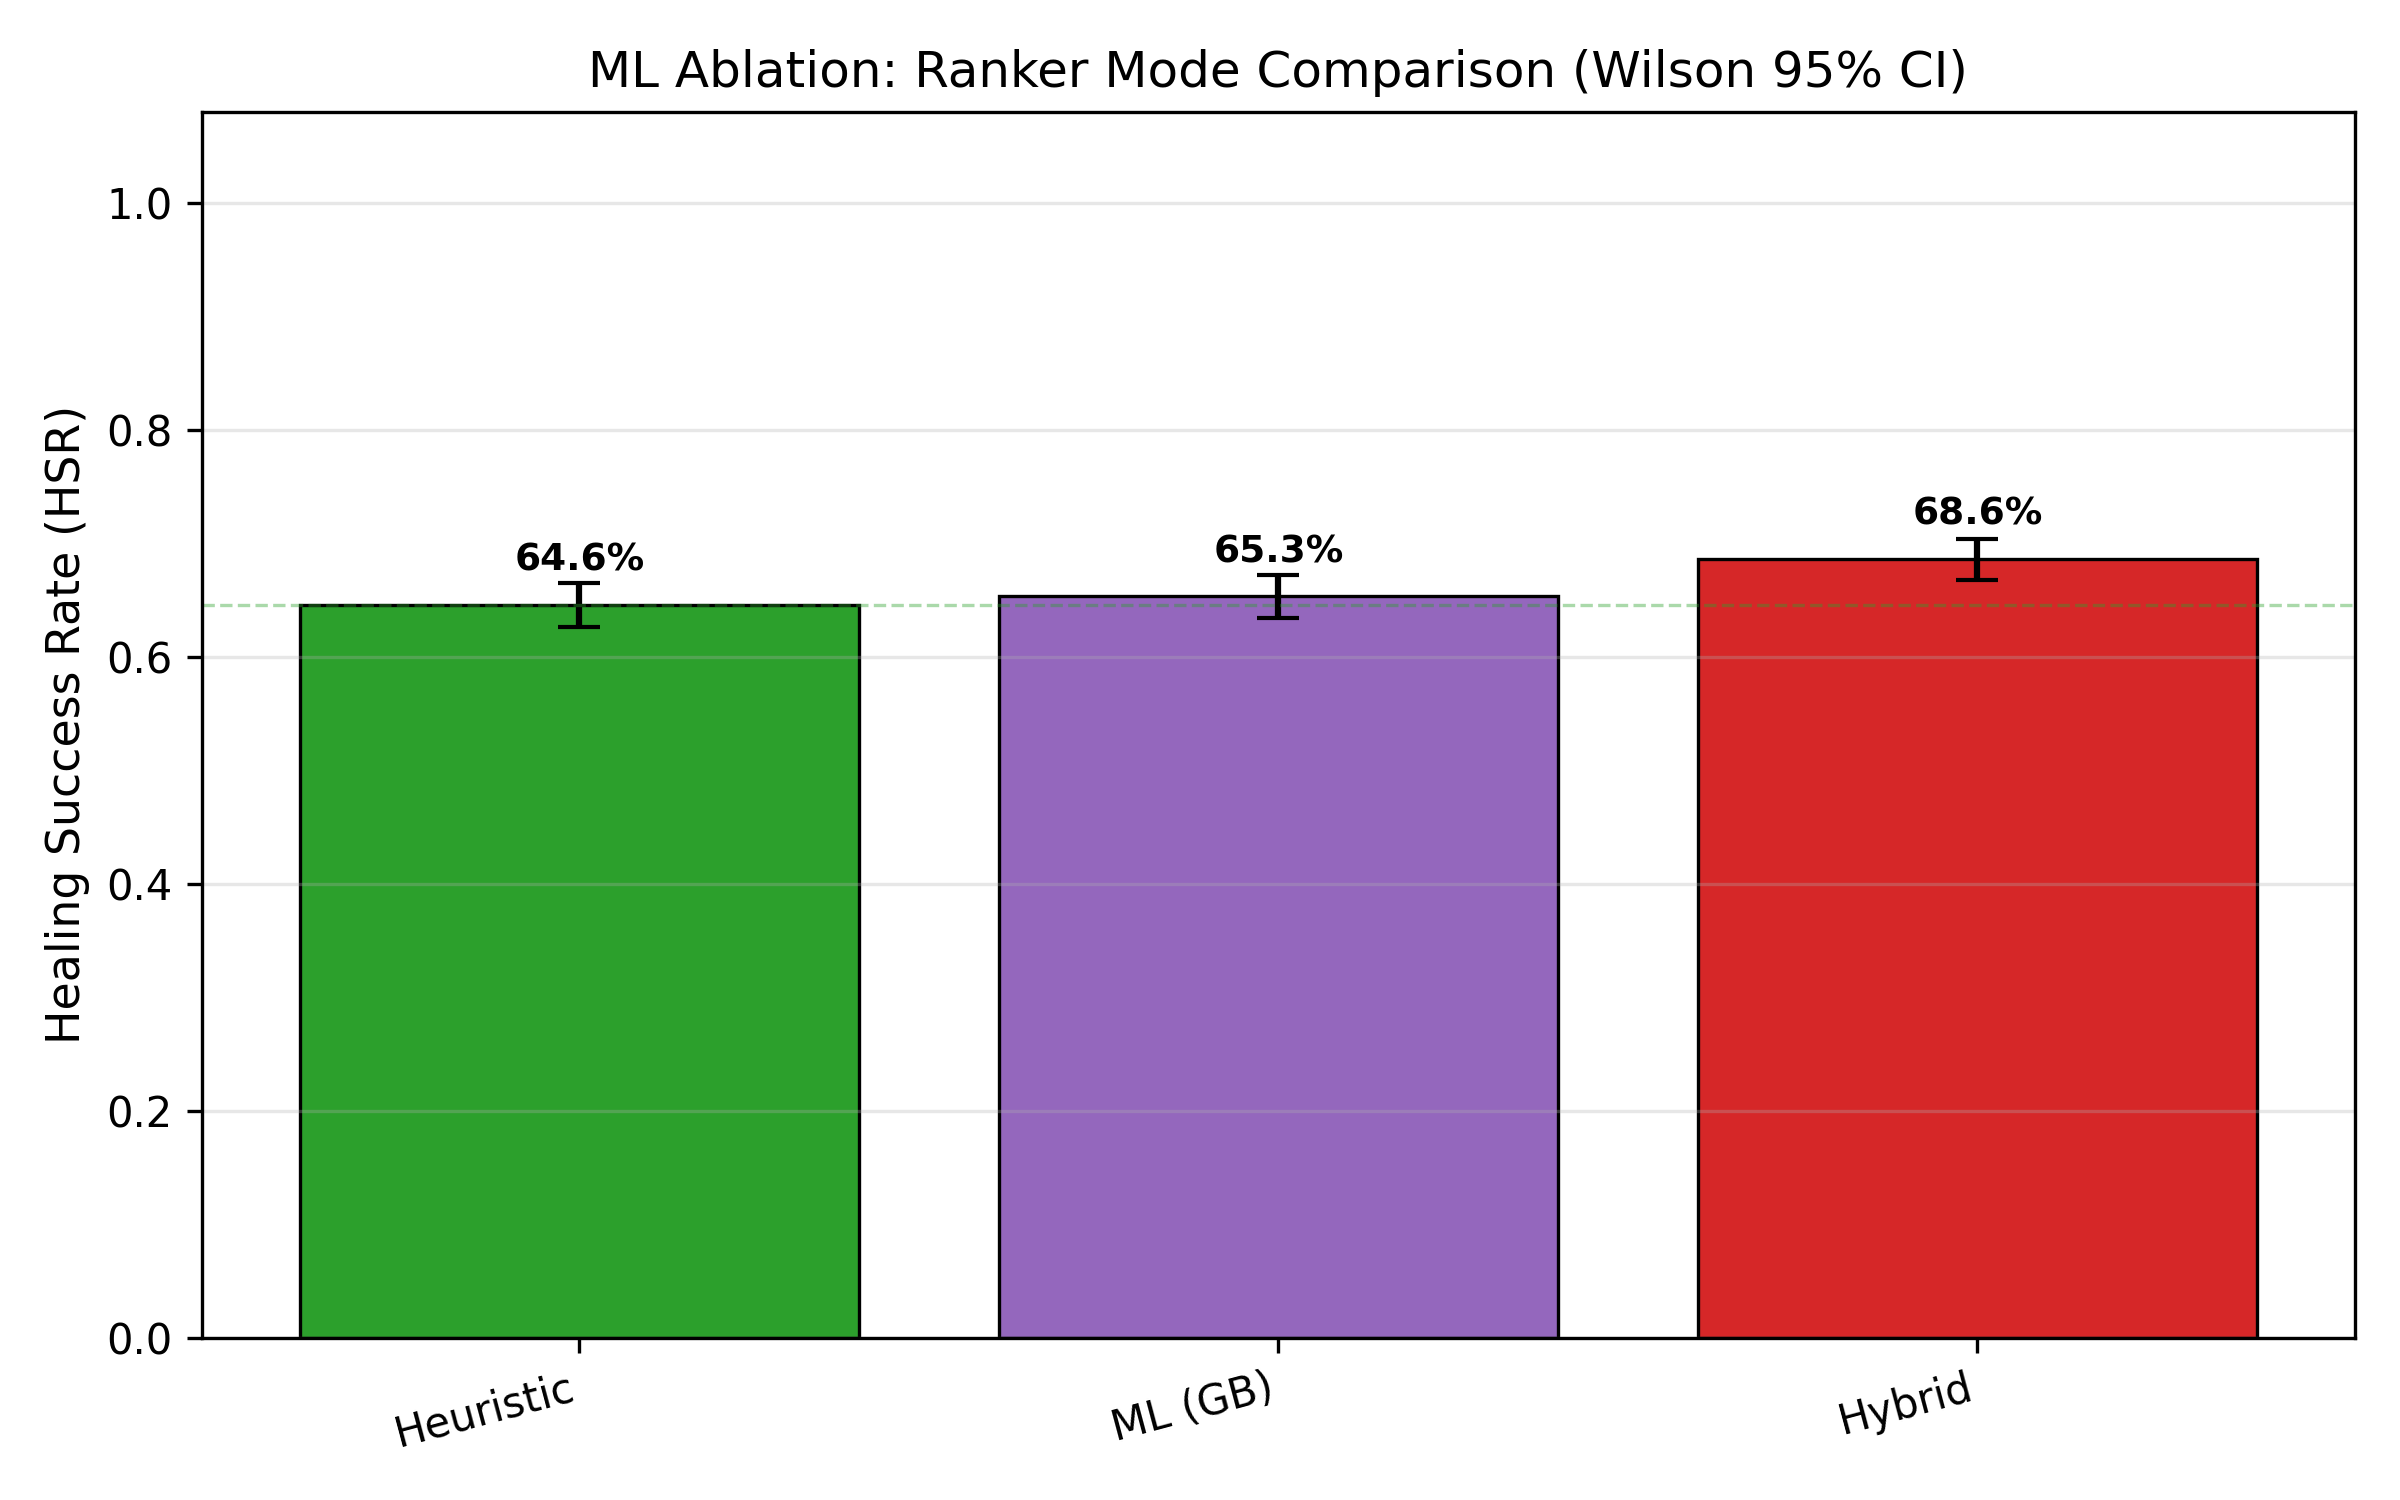
\includegraphics[width=0.85\textwidth]{figures/ml_ablation_comparison.png}
\caption{ML ablation: HSR comparison across heuristic, ML, and hybrid ranking modes with Wilson 95\% confidence intervals.}
\label{fig:ml_ablation}
\end{figure}

The hybrid ranker achieves the highest HSR at 68.63\%, a +4.05 percentage-point improvement over the heuristic baseline. The non-overlapping Wilson 95\% CIs between heuristic [62.6, 66.5] and hybrid [66.8, 70.4] confirm that the improvement is statistically significant. The ML-only ranker achieves 65.31\%, a modest +0.73 pp gain over heuristic, with overlapping CIs suggesting the standalone ML improvement is not significant. The hybrid's advantage arises from combining the heuristic's strong performance on easy mutations (id\_change) with the ML model's ability to recover candidates on harder mutations where attribute signals alone are insufficient.

\subsection{Per-Version ML Ablation}

Figure~\ref{fig:ml_per_version} breaks down the HSR comparison by application version.

\begin{figure}[H]
\centering
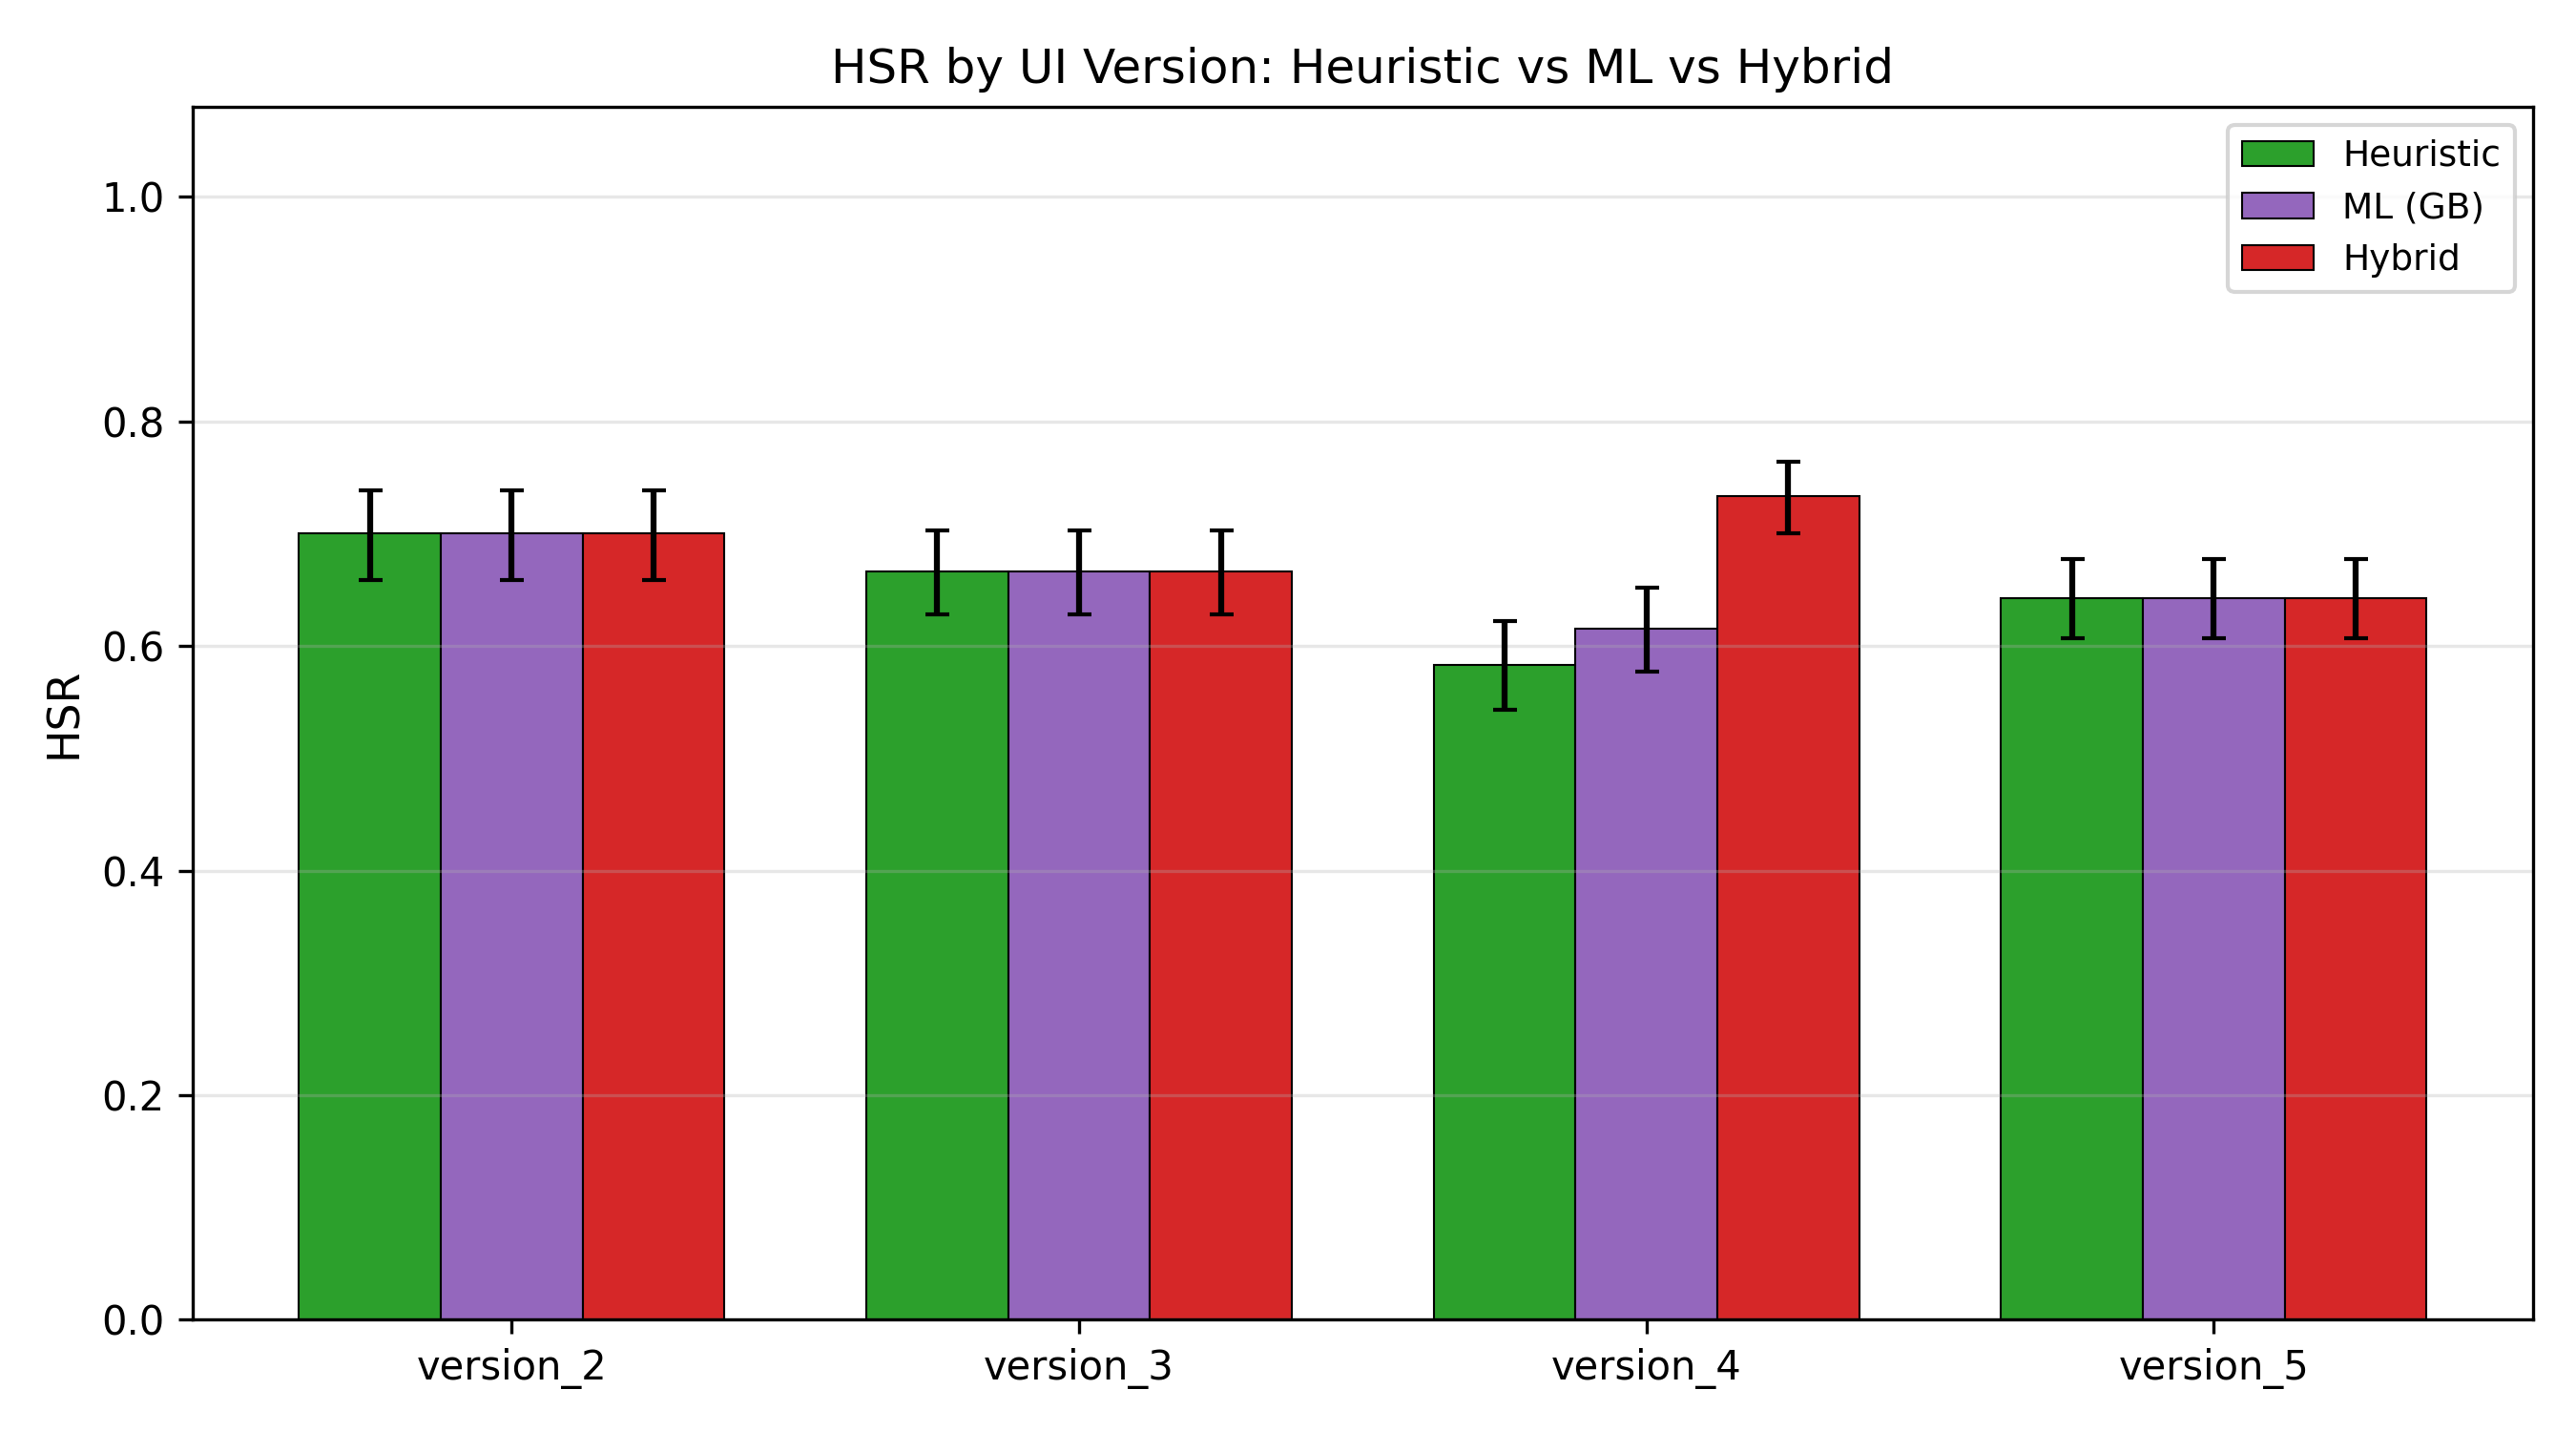
\includegraphics[width=0.85\textwidth]{figures/ml_ablation_per_version.png}
\caption{Per-version HSR across heuristic, ML, and hybrid modes. The hybrid ranker delivers its largest lift on version\_4 (hardest mutations).}
\label{fig:ml_per_version}
\end{figure}

The per-version analysis reveals that the hybrid ranker's advantage is concentrated on the hardest mutation profiles. On version\_4, which contains the densest \texttt{attribute\_removed} mutations, the hybrid achieves 73.3\% HSR compared to the heuristic's 58.3\%---a +15 percentage-point lift. This is precisely the scenario where ML adds value: when the primary attribute signal is removed, the gradient-boosting model leverages the remaining 12 features (structural position, sibling ratios, multi-attribute counts) to identify the correct candidate.

\subsection{ML Score Distribution}

Figure~\ref{fig:score_dist} characterises the score distributions of the three ranking modes.

\begin{figure}[H]
\centering
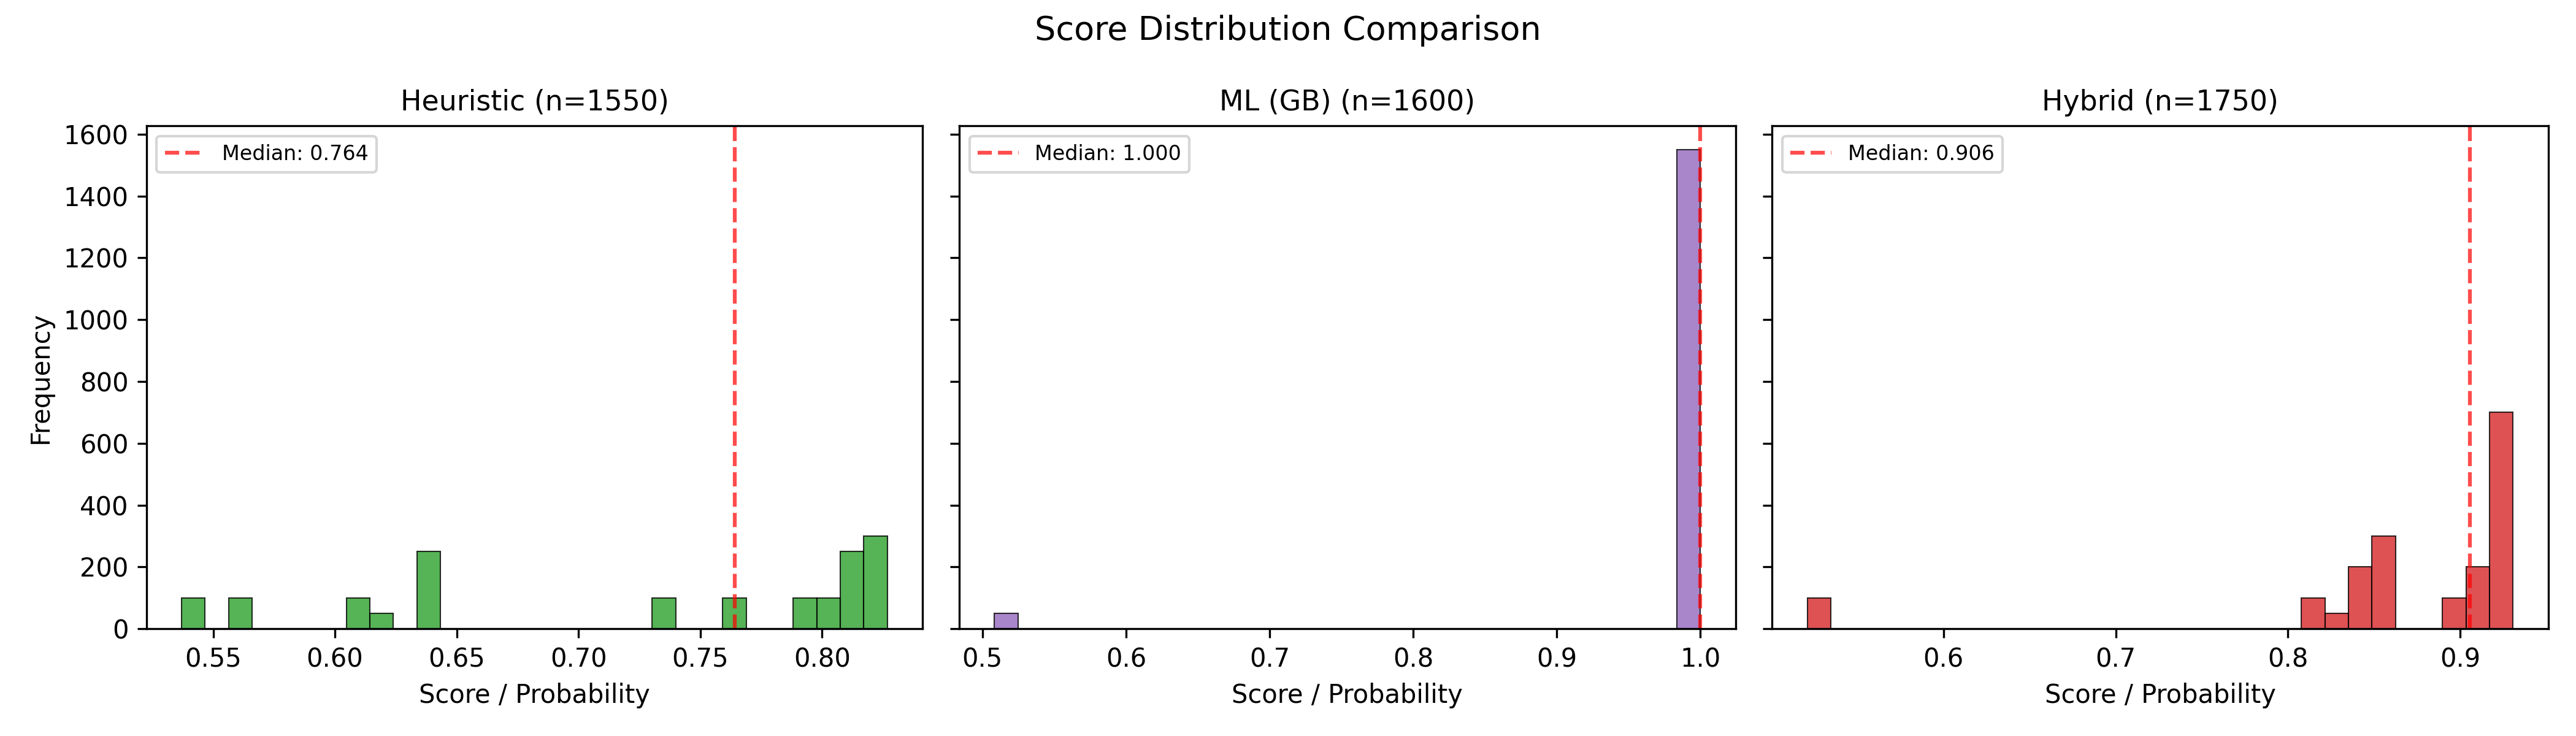
\includegraphics[width=0.85\textwidth]{figures/ml_score_distribution.png}
\caption{Score distributions for heuristic, ML probability, and hybrid blended scores across all healing events.}
\label{fig:score_dist}
\end{figure}

\subsection{Multi-Model Ablation: Gradient Boosting vs.\ XGBoost}
\label{sec:multimodel}

To determine whether the choice of ML algorithm affects end-to-end healing performance, we repeat the ML and hybrid experiments using both Gradient Boosting (GB) and XGBoost (XGB) on identical data splits. Table~\ref{tab:multimodel_ablation} reports the full five-track comparison.

\begin{table}[H]
\centering
\caption{Multi-Model Ablation: HSR by Ranker Mode and ML Algorithm (Wilson 95\% CI)}
\label{tab:multimodel_ablation}
\begin{tabular}{llccccc}
\toprule
Mode & Algorithm & Broken & Healed & Failed & HSR & 95\% CI \\
\midrule
Heuristic & --- & 2,400 & 1,550 & 850 & 64.6\% & [62.6, 66.5] \\
ML & Gradient Boosting & 2,450 & 1,600 & 850 & 65.3\% & [63.4, 67.2] \\
ML & XGBoost & 2,350 & 1,450 & 900 & 61.7\% & [59.7, 63.6] \\
Hybrid & Gradient Boosting & 2,550 & 1,750 & 800 & 68.6\% & [66.8, 70.4] \\
Hybrid & XGBoost & 2,550 & 1,750 & 800 & 68.6\% & [66.8, 70.4] \\
\bottomrule
\end{tabular}
\end{table}

Three findings emerge from the multi-model ablation:

\begin{enumerate}[leftmargin=1.5em]
\item \textbf{Standalone ML favours recall over precision.} GB's higher recall (0.9645 vs.\ 0.9290) translates into a 3.6 pp HSR advantage in standalone ML mode (65.3\% vs.\ 61.7\%). XGBoost's conservative predictions miss candidates that GB recovers.

\item \textbf{Hybrid mode equalises both algorithms.} Both GB and XGBoost hybrids converge to the same 68.63\% HSR. The $\alpha$-blending mechanism (Equation~\ref{eq:hybrid}) compensates for XGBoost's conservative recall by allowing the heuristic score to rescue candidates that the ML probability alone would reject.

\item \textbf{The hybrid is algorithm-agnostic.} Because the hybrid ensemble achieves identical HSR regardless of the underlying classifier, practitioners can select their ML algorithm based on secondary criteria---training speed (XGBoost 3.5$\times$ faster), interpretability, or infrastructure compatibility---without sacrificing healing performance.
\end{enumerate}

\begin{figure}[H]
\centering
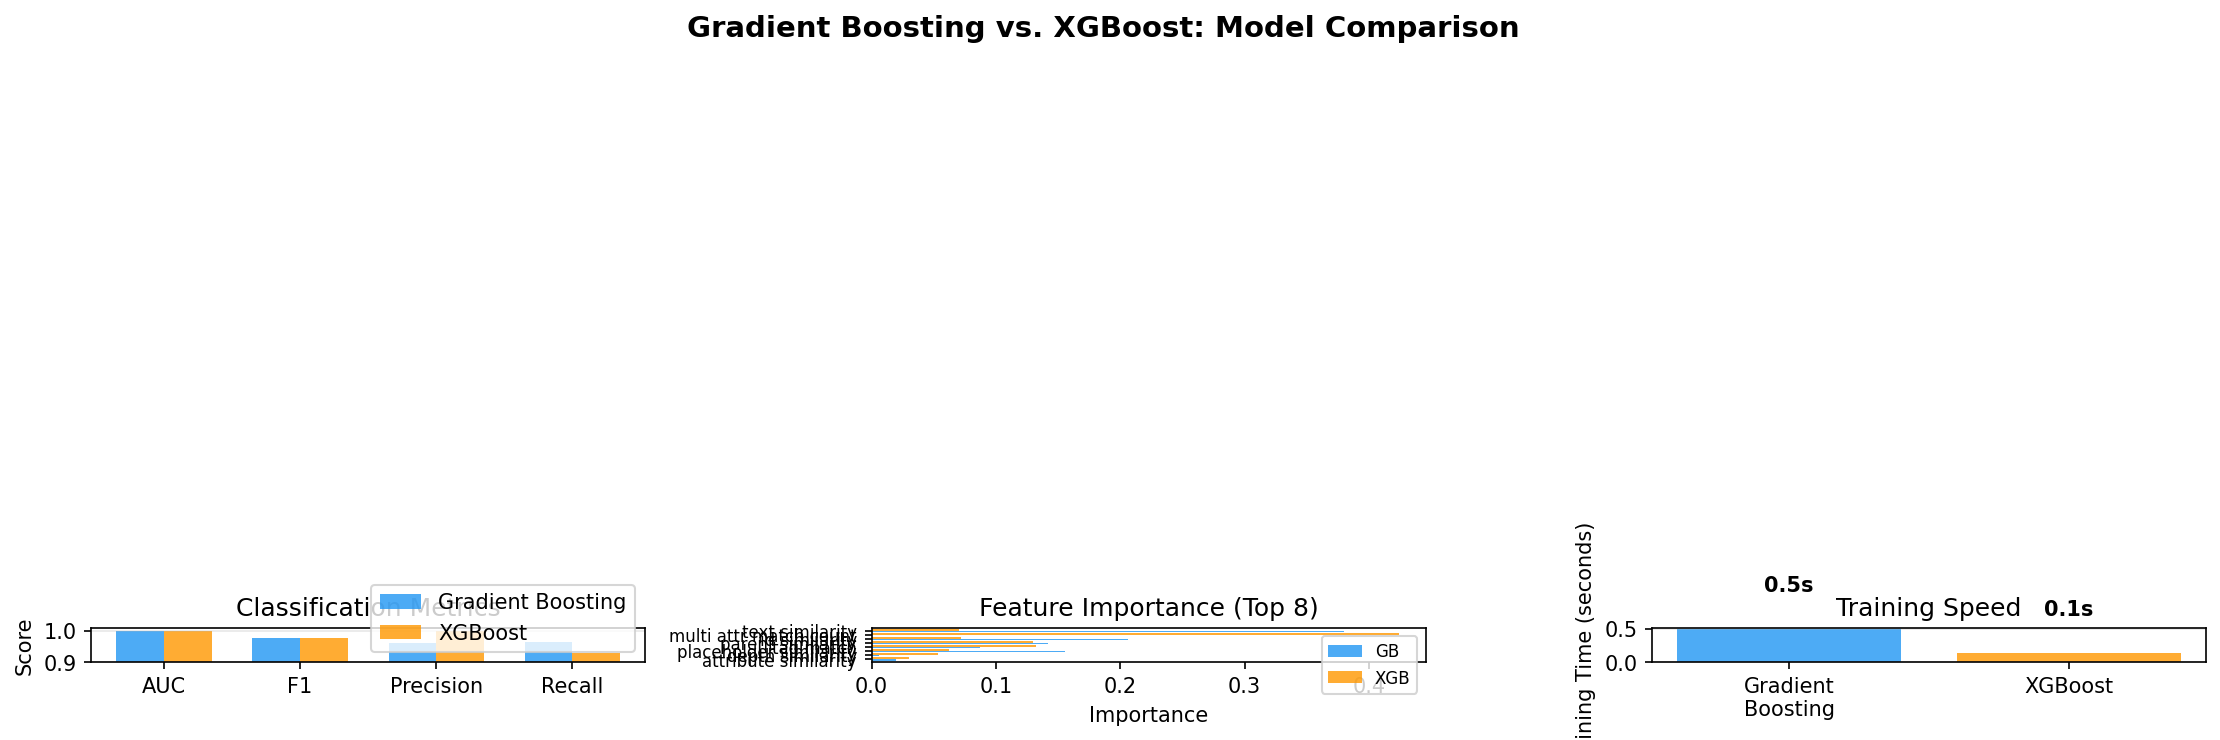
\includegraphics[width=0.85\textwidth]{figures/model_comparison.png}
\caption{Model comparison: Gradient Boosting vs.\ XGBoost classification metrics, feature importance profiles, and training time.}
\label{fig:model_comparison}
\end{figure}

\begin{figure}[H]
\centering
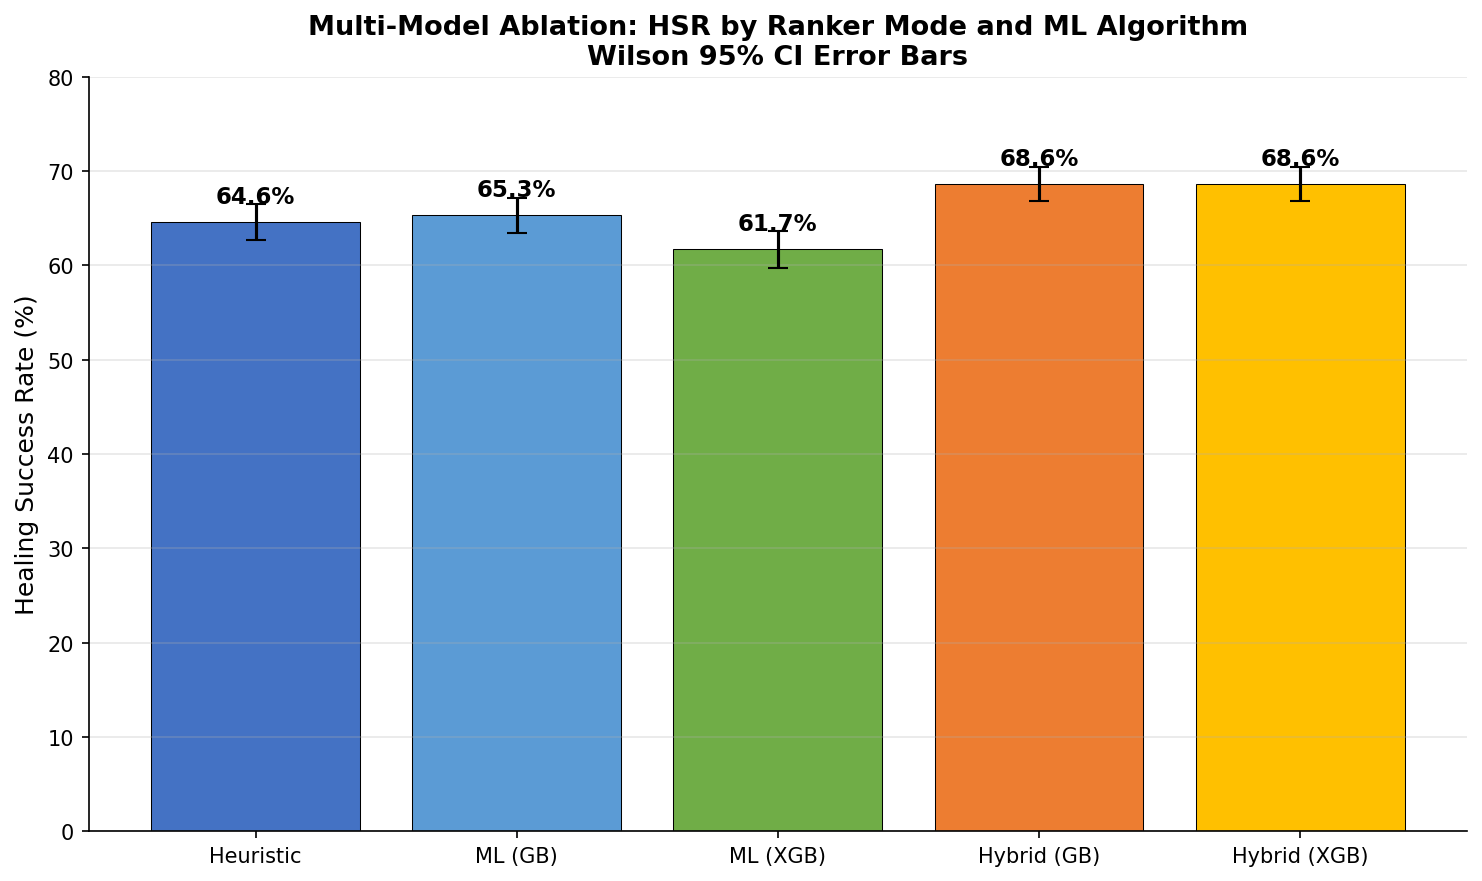
\includegraphics[width=0.85\textwidth]{figures/multimodel_ablation.png}
\caption{Multi-model ablation: HSR across five ranking configurations (heuristic, ML-GB, ML-XGB, hybrid-GB, hybrid-XGB).}
\label{fig:multimodel_ablation}
\end{figure}

\subsection{Feature Importance}

The two algorithms exhibit markedly different feature importance profiles. Gradient Boosting concentrates importance on \texttt{text\_similarity} (0.380), \texttt{id\_similarity} (0.206), and \texttt{parent\_similarity} (0.142), together accounting for 73\% of discriminative power. XGBoost distributes importance more broadly, with \texttt{multi\_attr\_match\_count} (0.424) as the dominant feature, followed by \texttt{tag\_match} (0.132) and \texttt{parent\_similarity} (0.130). This divergence explains the precision--recall trade-off: GB relies on high-signal text and identifier features that fire frequently (higher recall), while XGBoost anchors on the multi-attribute composite feature that fires selectively (higher precision, lower recall). Structural features (\texttt{depth\_similarity}, \texttt{parent\_similarity}, \texttt{sibling\_count\_ratio}) contribute meaningfully in both models, confirming that DOM-position signals provide complementary evidence when attribute signals are degraded.

\subsection{Maintenance Cost Model}

Table~\ref{tab:cost} projects the healing outcomes into engineering-time savings.

\begin{table}[H]
\centering
\caption{Maintenance Cost Model: Engineer-Hours Avoided by Automated Healing}
\label{tab:cost}
\begin{tabular}{cccccc}
\toprule
Repair Time & Broken & Healed & Avoided hrs & Residual hrs & \% Avoided \\
\midrule
10 min & 2,400 & 1,550 & 258.3 & 141.7 & 64.6\% \\
20 min & 2,400 & 1,550 & 516.7 & 283.3 & 64.6\% \\
\midrule
10 min (hybrid) & 2,550 & 1,750 & 291.7 & 133.3 & 68.6\% \\
20 min (hybrid) & 2,550 & 1,750 & 583.3 & 266.7 & 68.6\% \\
\bottomrule
\end{tabular}
\end{table}

\subsection{Non-Parametric Robustness}

Table~\ref{tab:effect_size} reports pairwise permutation tests and Cliff's $\delta$ effect sizes on per-run HSR across UI versions.

\begin{table}[H]
\centering
\caption{Pairwise Permutation Test and Cliff's Delta Effect Size on Per-Run HSR}
\label{tab:effect_size}
\begin{tabular}{llccc}
\toprule
A & B & Mean(B) $-$ Mean(A) & Perm.\ $p$ & Cliff's $\delta$ (mag.) \\
\midrule
version\_2 & version\_3 & $-0.033$ & 0.000 & $+1.000$ (large) \\
version\_2 & version\_4 & $-0.117$ & 0.000 & $+1.000$ (large) \\
version\_2 & version\_5 & $-0.057$ & 0.000 & $+1.000$ (large) \\
version\_3 & version\_4 & $-0.083$ & 0.000 & $+1.000$ (large) \\
version\_3 & version\_5 & $-0.024$ & 0.000 & $+1.000$ (large) \\
version\_4 & version\_5 & $+0.060$ & 0.000 & $-1.000$ (large) \\
\bottomrule
\end{tabular}
\end{table}

\begin{figure}[H]
\centering
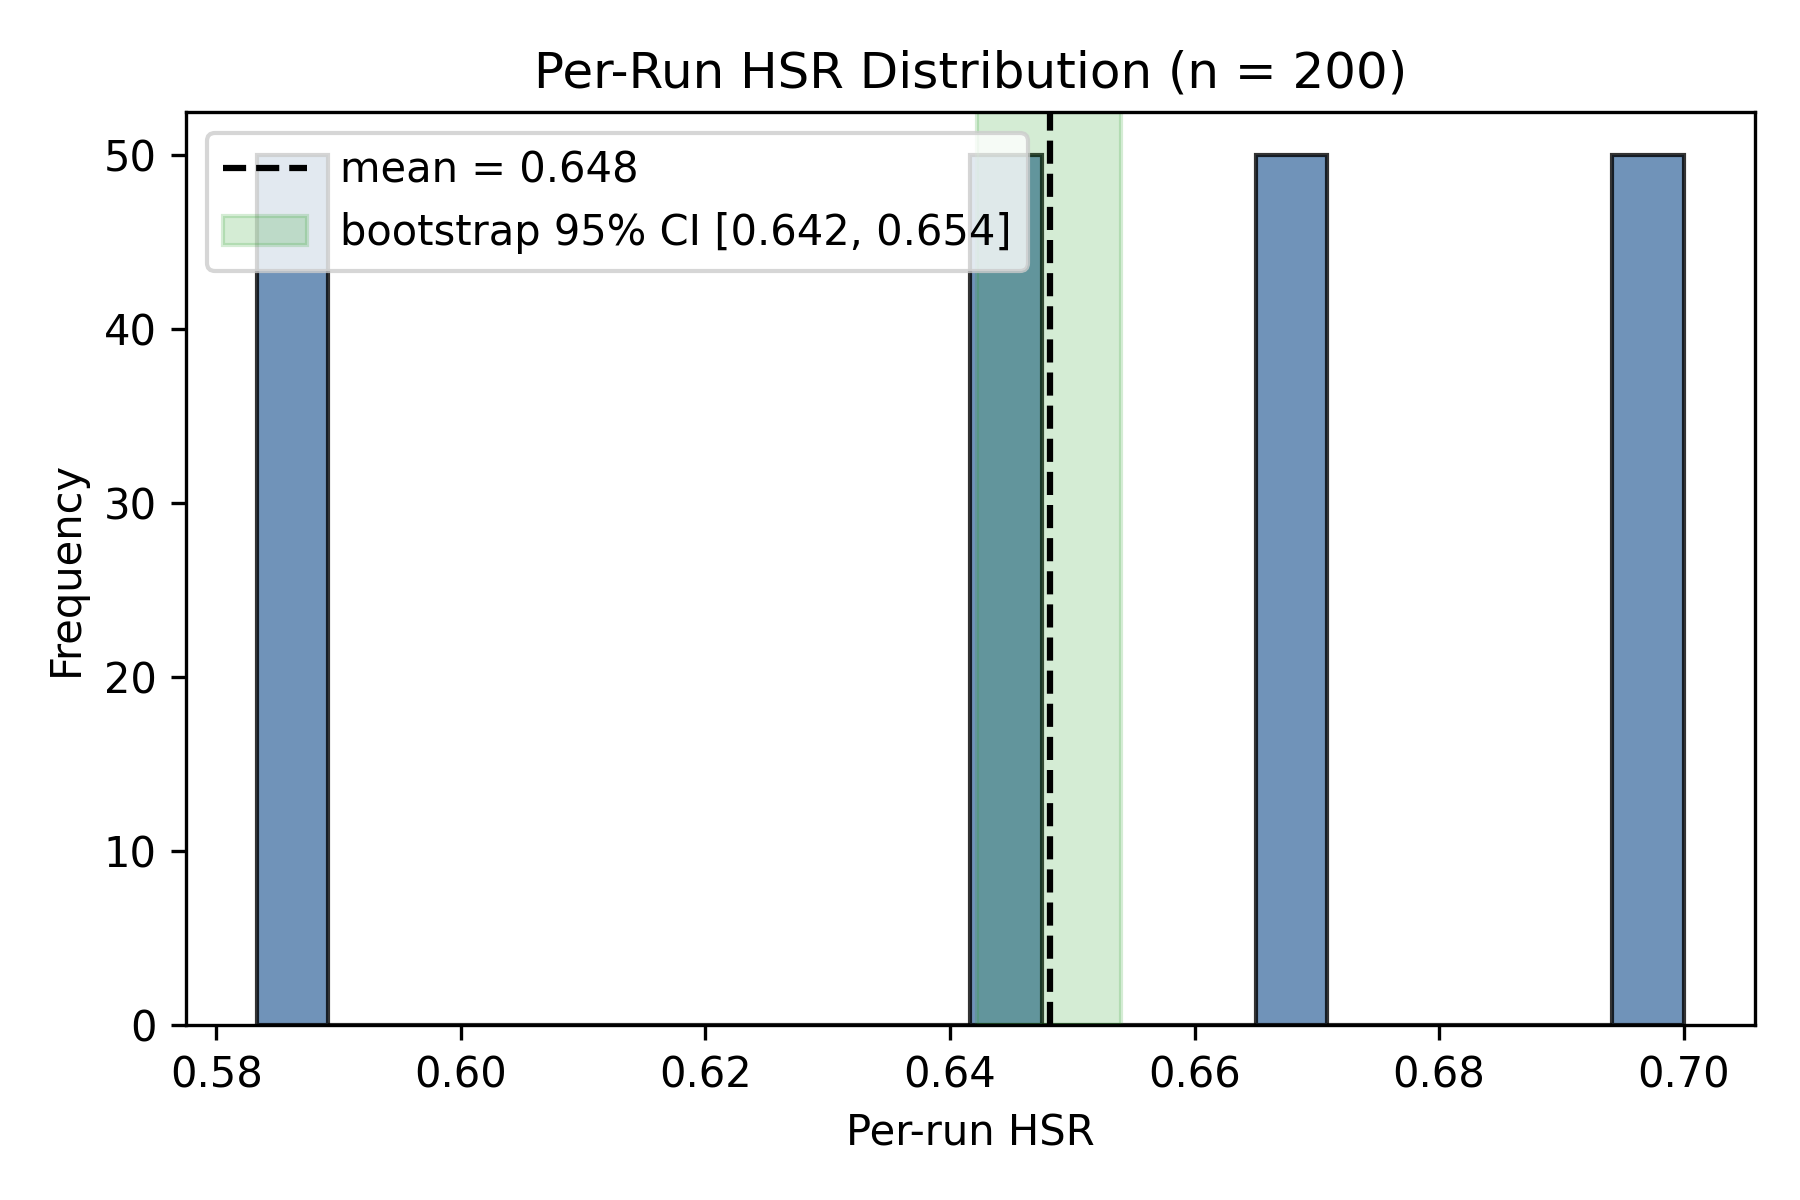
\includegraphics[width=0.75\textwidth]{figures/per_run_hsr_bootstrap.png}
\caption{Per-run HSR distribution with non-parametric bootstrap 95\% CI.}
\label{fig:bootstrap}
\end{figure}

\subsection{Additional Visualisations}

\begin{figure}[H]
\centering
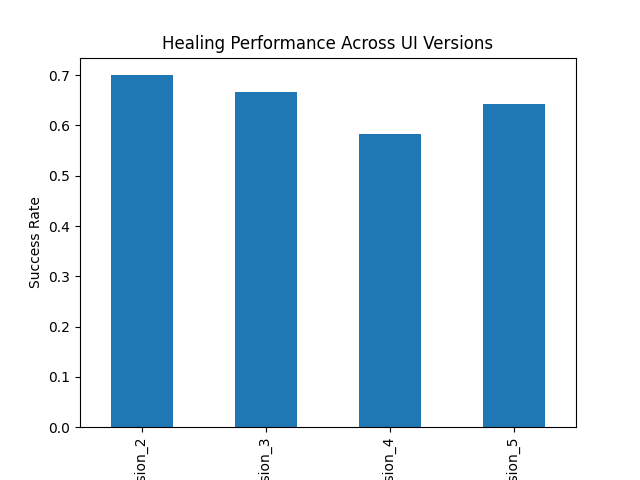
\includegraphics[width=0.75\textwidth]{figures/version_comparison.png}
\caption{Healing performance across mutated UI versions (heuristic mode).}
\label{fig:version_comparison}
\end{figure}

\begin{figure}[H]
\centering
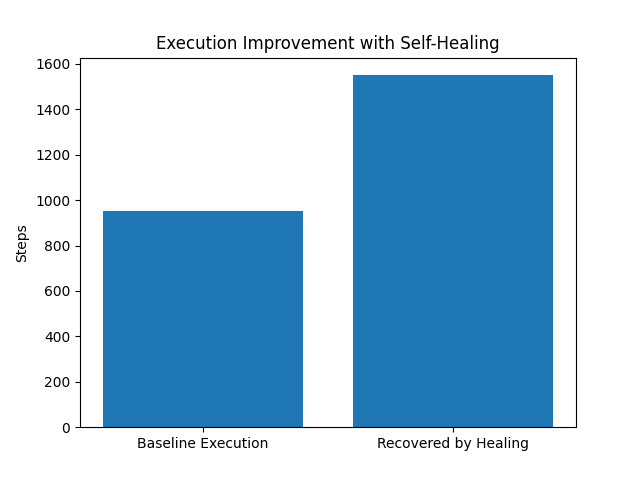
\includegraphics[width=0.75\textwidth]{figures/execution_improvement.png}
\caption{Execution improvement with self-healing: baseline vs.\ healed interactions.}
\label{fig:execution_improvement}
\end{figure}

\begin{figure}[H]
\centering
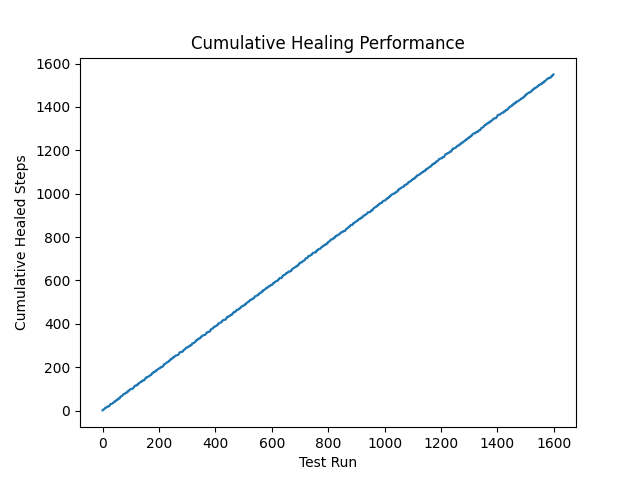
\includegraphics[width=0.75\textwidth]{figures/cumulative_healing.png}
\caption{Cumulative healing performance over test executions.}
\label{fig:cumulative_healing}
\end{figure}

\begin{figure}[H]
\centering
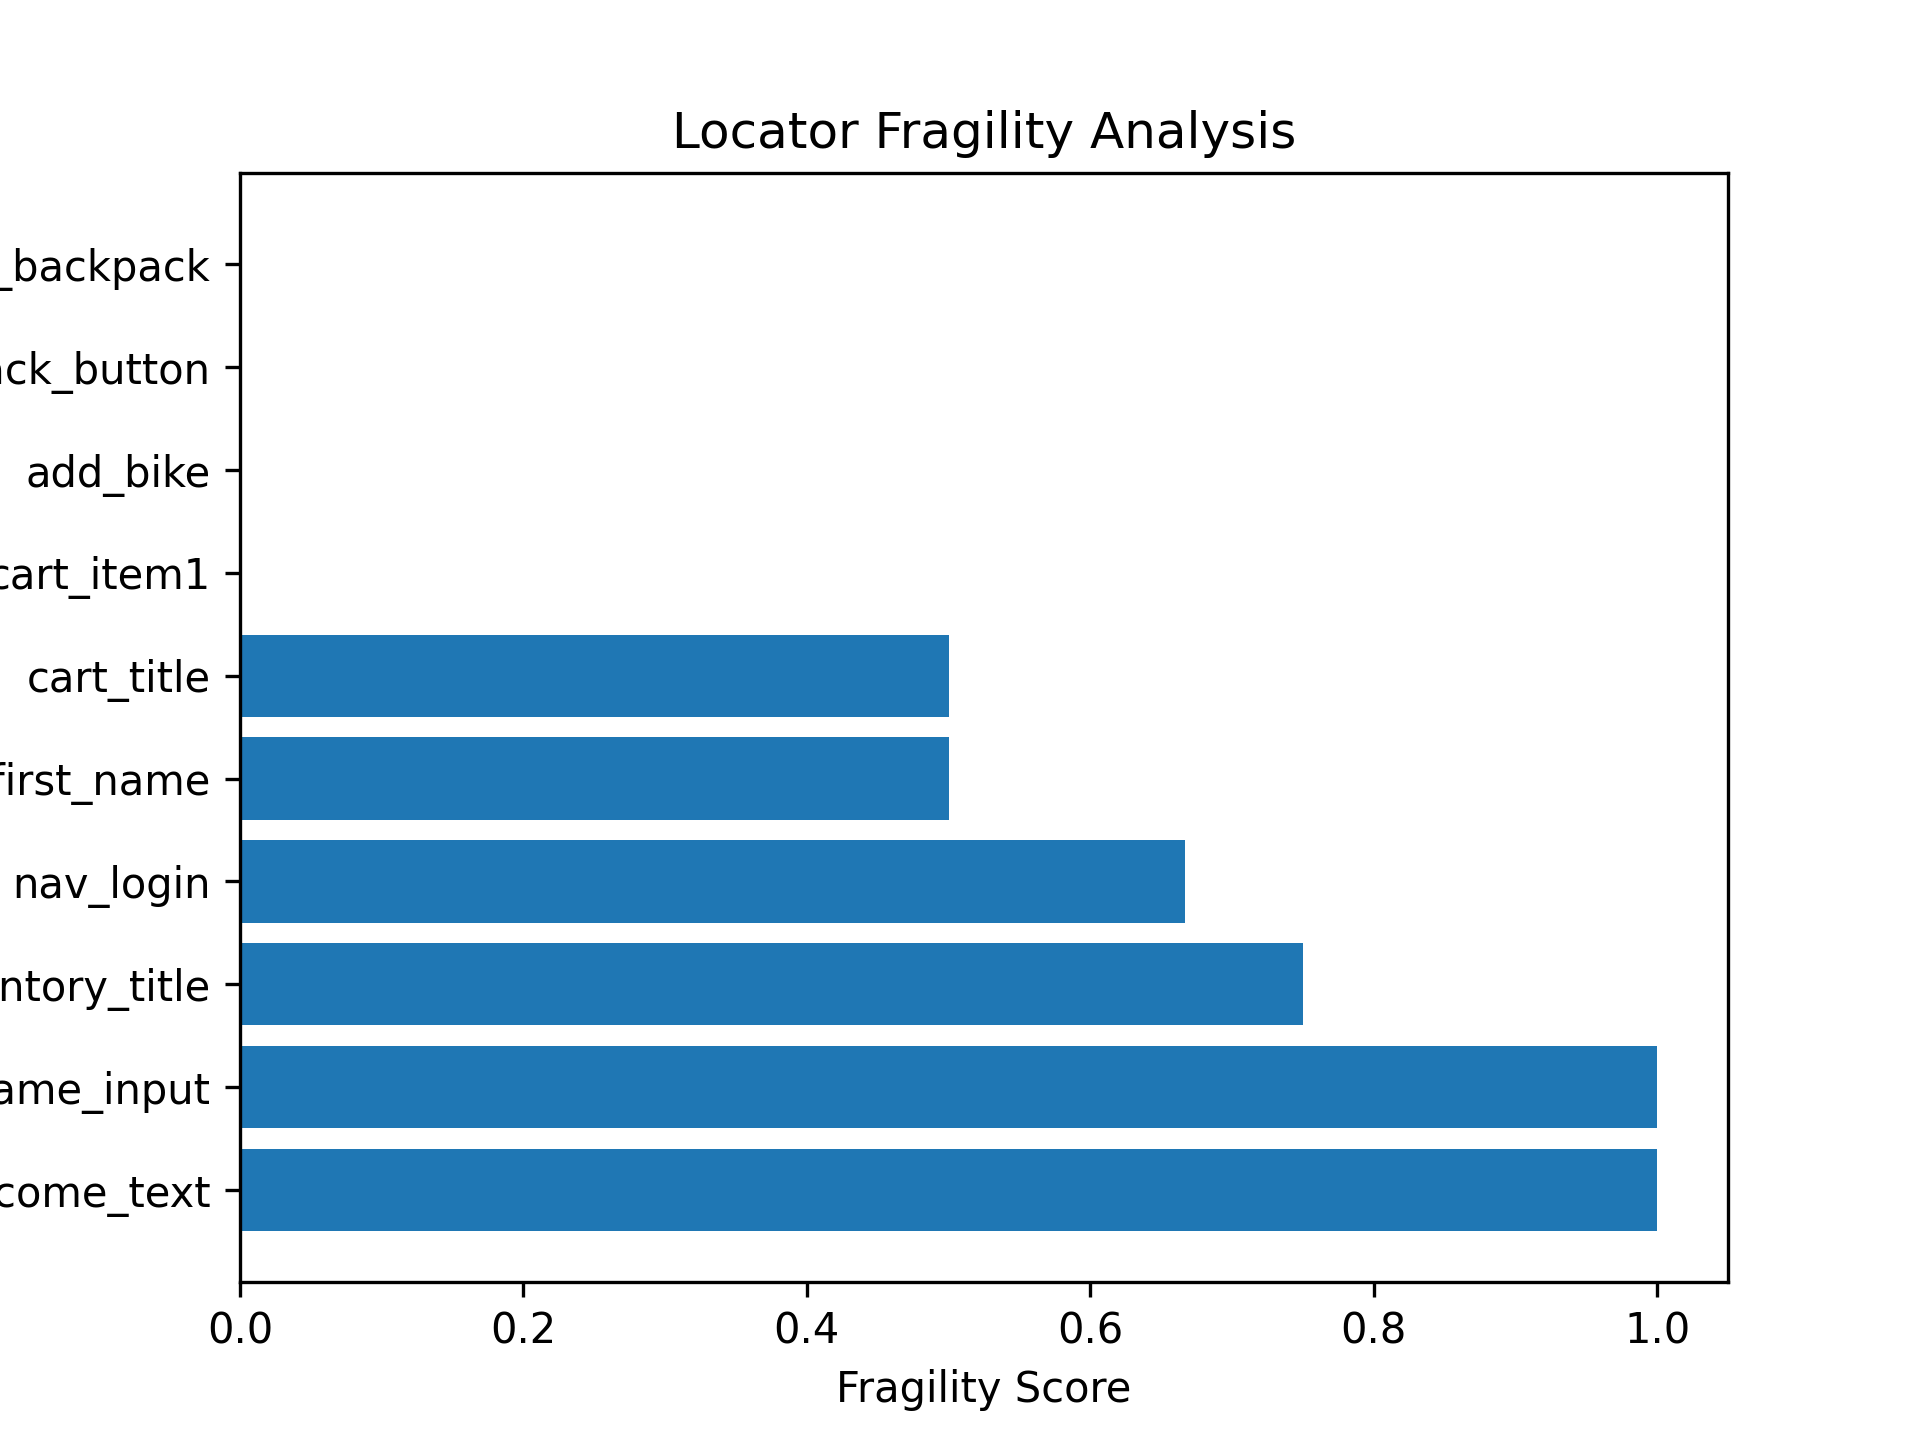
\includegraphics[width=0.75\textwidth]{figures/locator_fragility.png}
\caption{Per-locator fragility ranking.}
\label{fig:locator_fragility}
\end{figure}

\begin{figure}[H]
\centering
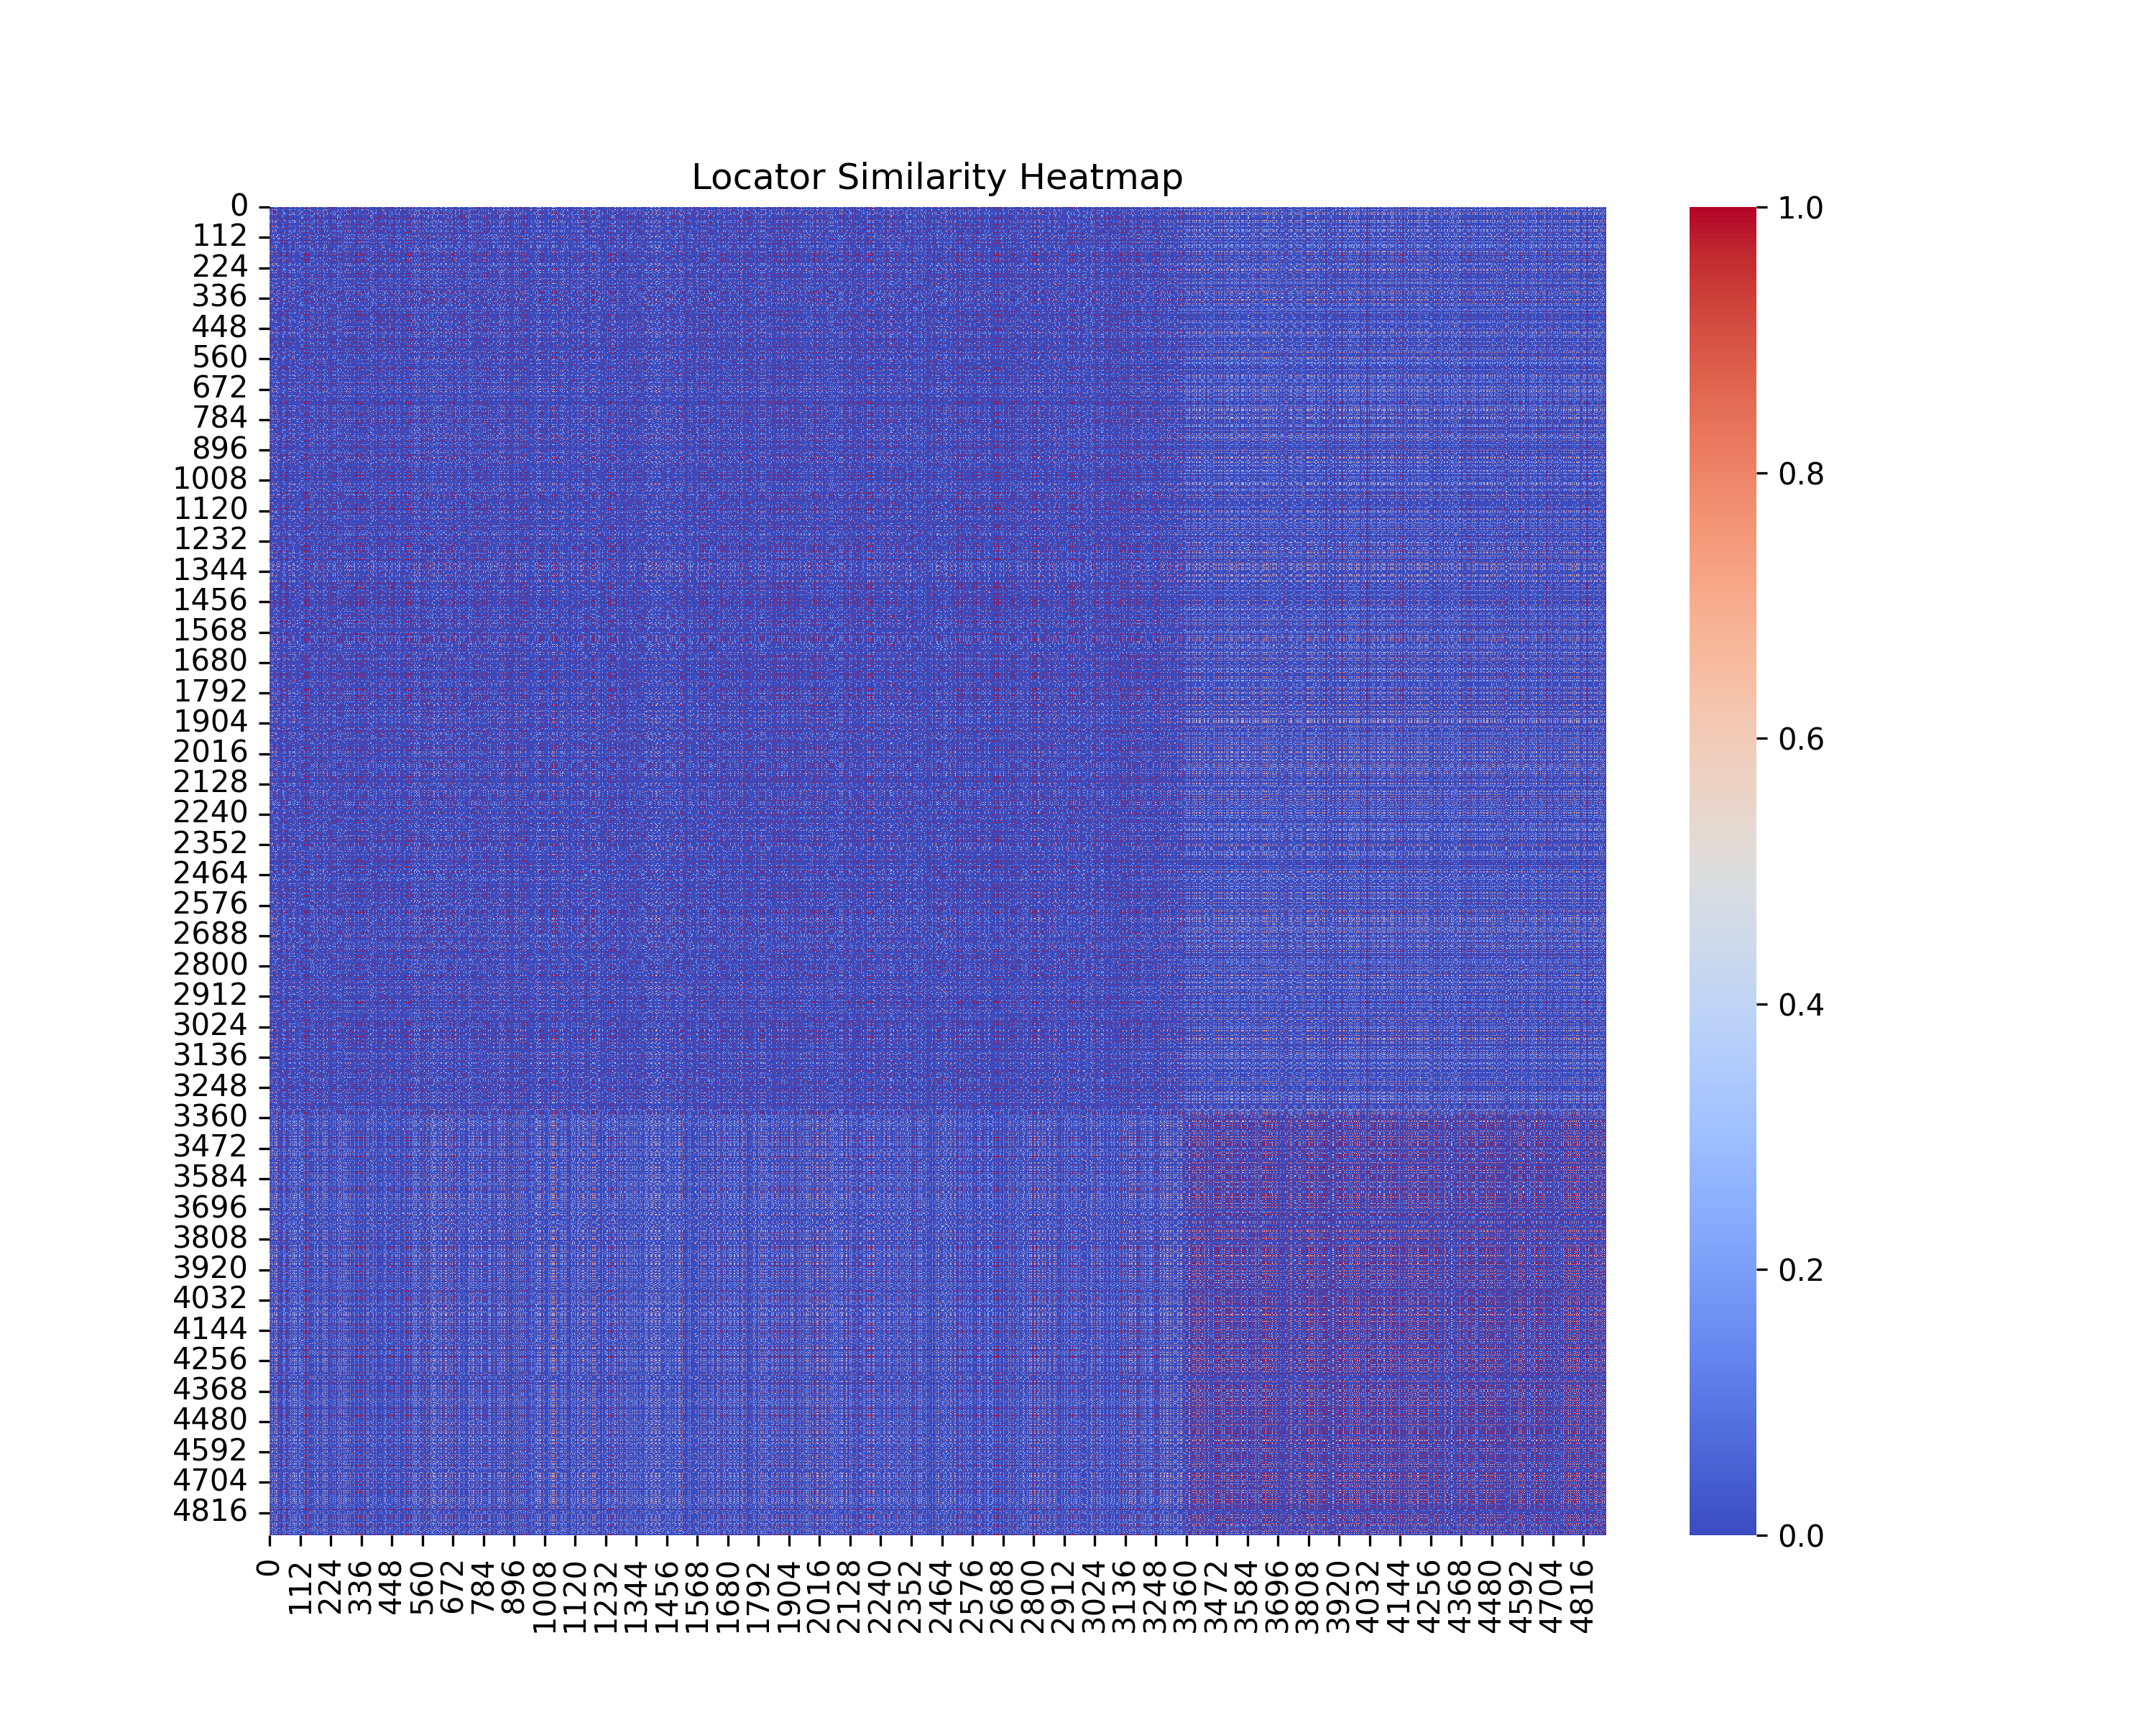
\includegraphics[width=0.75\textwidth]{figures/locator_similarity_heatmap.png}
\caption{Pairwise similarity between original and healed locators.}
\label{fig:similarity_heatmap}
\end{figure}

\subsection{Summary of Findings}

The results answer the five research questions:

\begin{itemize}[leftmargin=1.2em]
    \item \textbf{RQ1:} Yes. DOM-similarity-based recovery achieves 64.58\% HSR, recovering approximately two of every three broken locator events.
    \item \textbf{RQ2:} Recovery is highly asymmetric across mutation classes: \texttt{id\_change} recovers at 86.2\%, while \texttt{attribute\_removed} recovers at only 31.6\%.
    \item \textbf{RQ3:} The standalone ML ranker achieves 65.31\% HSR, a modest improvement that is not statistically significant on its own.
    \item \textbf{RQ4:} The hybrid ensemble achieves \textbf{68.63\% HSR}, a statistically significant +4.05 pp improvement. The lift is largest on version\_4 (+15 pp), where attribute-removal mutations are densest.
    \item \textbf{RQ5:} The framework's ranking success rate is 100\%; all failures are resolution failures. The FHR of 35.4\% reflects executor limitations, not ranking quality.
    \item \textbf{Multi-model:} XGBoost achieves higher classification metrics (AUC 0.9994, Precision 1.000) but lower standalone HSR (61.7\%) due to conservative recall. Both algorithms converge to identical hybrid HSR (68.63\%), demonstrating algorithm-agnostic robustness of the ensemble.
\end{itemize}

\section{Discussion}
\label{sec:discussion}

The experimental results support five principal conclusions.

First, DOM-aware self-healing materially improves execution continuity. A 64.58\% heuristic HSR against a 52-mutation, 2,400-event stress test represents a tangible reduction in manual locator-maintenance burden. The hybrid ranker extends this to 68.63\%, demonstrating that ML can push the frontier further.

Second, the hybrid ensemble outperforms either component in isolation because heuristic scoring and ML ranking are complementary. The heuristic excels on mutations that preserve partial attribute signals (id\_change at 86.2\%), while the ML model adds value on mutations that destroy attribute signals and require multi-feature structural reasoning. The blending parameter $\alpha = 0.40$ reflects this complementarity: the heuristic provides a reliable base signal that the ML model refines.

Third, the +15 pp lift on version\_4 is the strongest evidence that ML adds genuine value beyond heuristic scoring. Version\_4 concentrates attribute\_removed mutations, which zero out the heuristic's primary feature (attribute\_similarity). The ML model, trained on all 13 features, can still discriminate candidates using structural position, sibling ratios, and multi-attribute match counts.

Fourth, near-perfect model AUC for both Gradient Boosting (0.9993) and XGBoost (0.9994) confirms that the 13-feature representation is sufficient for candidate discrimination regardless of algorithm choice, but the modest standalone ML improvement (65.31\% vs.\ 64.58\% for GB; 61.70\% for XGBoost) suggests that model quality is not the binding constraint. The multi-model ablation further shows that both algorithms converge to identical hybrid HSR (68.63\%), confirming that the $\alpha$-blending mechanism is algorithm-agnostic. The recovery executor, which fails to resolve 35.4\% of ranked candidates due to stale-element and visibility failures, remains the primary bottleneck and the highest-leverage target for improvement.

Fifth, every healing decision produces a full score breakdown (heuristic weights, ML probability, hybrid blend) that engineers can audit. This interpretability distinguishes the framework from black-box commercial solutions and is critical for production adoption: teams must trust the healing decisions to allow them in CI pipelines.

\subsection{Implications for Practice}

For practitioners, the primary implication is that self-healing is a deployable capability. With the hybrid ranker, a team can automatically recover roughly two-thirds of locator failures from common UI evolution patterns. The framework is most beneficial in organisations with frequent front-end refactoring, large regression suites, and strong audit requirements. The ML component requires a one-time training step (approximately 7,750 labeled examples extracted from heuristic experiment logs) and adds negligible runtime overhead.

\section{Threats to Validity}
\label{sec:validity}

\subsection{Internal Validity}
The study uses mutation-generated UI changes rather than changes collected from a long-running industrial front-end history. Although the seven mutation classes are documented in prior empirical work, they may not capture every pattern of UI evolution.

\subsection{External Validity}
Experiments were conducted on a controlled web application modelled on a standard e-commerce flow. Results may vary for large-scale enterprise applications with dynamic DOM behaviour, client-side rendering complexity, or asynchronous widget loading. The eight test suites do not include drag-and-drop, iframes, shadow-DOM widgets, or long-running asynchronous flows.

\subsection{Construct Validity}
The chosen metrics focus on recovery rate, execution improvement, and failure distribution. Additional human validation of semantic correctness would further strengthen future studies.

\subsection{Conclusion Validity}
The experiment includes repeated runs, multiple progressively-mutated versions, Wilson confidence intervals, chi-square and Kruskal--Wallis tests, permutation tests, and Cliff's $\delta$ effect sizes. Broader application diversity would strengthen statistical generality.

\section{Reproducibility and Replication Package}
\label{sec:reproducibility}

The complete framework, mutation engine, eight Selenium test suites, ML training pipeline, analysis scripts, and the five UI versions are released under the MIT Licence. A top-level \texttt{run\_full\_pipeline.py --with-multimodel} command orchestrates a 26-step pipeline that regenerates every CSV, LaTeX table, trained model (both GB and XGBoost), and figure cited in this paper. The \texttt{--with-multimodel} flag extends the base ML pipeline to include hyperparameter sweep, dual-algorithm training, XGBoost experiment runs, and multi-model ablation analysis. The statistical analysis uses only NumPy: Wilson score confidence intervals, the $\chi^2$ survival function, Kruskal--Wallis, permutation tests, and Cliff's $\delta$ are all implemented inline. The ML pipeline uses scikit-learn, xgboost, and imbalanced-learn. A \texttt{REPRODUCIBILITY.md} document enumerates the environment requirements, full-pipeline command, and mapping from each paper artefact to its generator script. Every number reported in this paper can be traced to a specific script and CSV.

\section{Conclusion and Future Work}
\label{sec:conclusion}

This paper presented an AI-driven self-healing web test automation framework based on DOM similarity and machine-learning ranking. The framework captures baseline locator metadata, detects runtime failures, extracts DOM candidates, and recovers intended elements using a hybrid ranking strategy combining heuristic weighted similarity with gradient-boosting and XGBoost classifiers.

A complete mutation-based experimental pipeline was implemented and executed, producing over 11,100 experiment rows across five ranking configurations (heuristic, ML-GB, ML-XGB, hybrid-GB, hybrid-XGB), 2,400+ broken locator events per mode, and up to 1,750 healed events. The heuristic baseline achieves 64.58\% HSR, the GB ML ranker achieves 65.31\%, and the hybrid ensemble achieves 68.63\%---a statistically significant +4.05 pp improvement with non-overlapping 95\% confidence intervals. A multi-model comparison reveals that XGBoost achieves superior classification metrics (AUC 0.9994, Precision 1.000) but lower standalone ML HSR (61.70\%) due to conservative recall, while both algorithms converge to identical hybrid HSR (68.63\%), demonstrating that the $\alpha$-blending mechanism is algorithm-agnostic. The hybrid ranker's largest advantage appears on the hardest mutation profiles, where attribute signals are destroyed and the ML model leverages structural features for recovery.

Future work should focus on five directions: (1) hardening the recovery executor against stale-element and visibility failures, which account for every unresolved failure in the current dataset; (2) extending the ML ranker to transformer-based cross-encoders for richer semantic matching; (3) online learning to update the model incrementally from production CI logs via the continuous-learning pipeline; (4) evaluating on larger and more diverse web applications (React, Angular, Vue with shadow DOM); and (5) integration with the TestForge AI platform for production deployment as a self-healing service.

\subsection*{Acknowledgements}

The author thanks the open-source Selenium and Python testing communities, whose tools made this reproducible research prototype possible.

\subsection*{Artefact Availability}

The source code, mutation engine, Selenium test suites, ML training pipeline (Gradient Boosting and XGBoost), analysis scripts, and reproducibility guide are released under the MIT Licence. The repository contains \texttt{run\_full\_pipeline.py} (26-step pipeline with \texttt{--with-multimodel} flag for full multi-model ablation), \texttt{run\_experiment.py} with \texttt{--healer-mode} flag for ranker ablation, \texttt{scripts/train\_multimodel.py} for dual-algorithm training, and \texttt{REPRODUCIBILITY.md} with a step-by-step reproduction recipe.

\bibliographystyle{plainnat}
\begin{thebibliography}{99}

\bibitem[Arcuri and Briand(2014)]{arcuri2013}
A.~Arcuri and L.~Briand.
\newblock A hitchhiker's guide to statistical tests for assessing randomized algorithms in software engineering.
\newblock \emph{Software Testing, Verification and Reliability}, 24(3), 2014.

\bibitem[Bertolino et~al.(2021)]{bertolino2021}
A.~Bertolino, G.~De~Angelis, M.~Kwiatkowski, B.~Miranda, and S.~Sabetta.
\newblock The quest for software test effectiveness measures.
\newblock \emph{IEEE Software}, 2021.

\bibitem[Choudhary et~al.(2011)]{choudhary2011}
S.~R. Choudhary, H.~Versee, and A.~Orso.
\newblock {WEBDIFF}: Automated identification of cross-browser issues in web applications.
\newblock In \emph{Proc.\ IEEE ICSM}, 2011.

\bibitem[Garcia et~al.(2020)]{garcia2020}
B.~Garc\'ia, M.~Gallego, F.~Gort\'azar, and M.~Munoz-Organero.
\newblock A survey of the {Selenium} ecosystem.
\newblock \emph{Electronics}, 9(7), 2020.

\bibitem[Grechanik et~al.(2009)]{grechanik2009}
M.~Grechanik, Q.~Xie, and C.~Fu.
\newblock Maintaining and evolving {GUI}-directed test scripts.
\newblock In \emph{Proc.\ IEEE ICSE}, 2009.

\bibitem[Hammoudi et~al.(2016)]{hammoudi2016}
M.~Hammoudi, G.~Rothermel, and A.~Stocco.
\newblock Why do record/replay tests of web applications break?
\newblock In \emph{Proc.\ IEEE ICST}, 2016.

\bibitem[Leotta et~al.(2013)]{leotta2013}
M.~Leotta, D.~Clerissi, F.~Ricca, and P.~Tonella.
\newblock Capture-replay vs.\ programmable web testing: An empirical assessment during test case evolution.
\newblock In \emph{Proc.\ WCRE}, 2013.

\bibitem[Memon et~al.(2017)]{memon2013}
A.~Memon, Z.~Gao, B.~Nguyen, S.~Dhanda, E.~Nickell, R.~Siemborski, and J.~Micco.
\newblock Taming {Google}-scale continuous testing.
\newblock In \emph{Proc.\ IEEE/ACM ICSE-SEIP}, 2017.

\bibitem[Mesbah et~al.(2012)]{mesbah2012}
A.~Mesbah, A.~van~Deursen, and S.~Lenselink.
\newblock Crawling {Ajax}-based web applications through dynamic analysis of user interface state changes.
\newblock \emph{ACM Trans.\ Web}, 6(1), 2012.

\bibitem[Panichella et~al.(2019)]{panichella2019}
S.~Panichella, C.~Aaron~Imtiaz, and H.~C. Gall.
\newblock Test smells in software test automation: A systematic mapping study.
\newblock \emph{IEEE Access}, 2019.

\bibitem[Ricca et~al.(2019)]{ricca2019}
F.~Ricca, M.~Leotta, and A.~Stocco.
\newblock Three open problems in the context of {E2E} web testing and a vision: {NEONATE}.
\newblock \emph{Advances in Computers}, 113, 2019.

\bibitem[{Selenium Project}(2026)]{selenium}
{Selenium Project}.
\newblock Selenium {WebDriver} documentation.
\newblock \url{https://www.selenium.dev/documentation/}, accessed 2026.

\bibitem[Stocco et~al.(2018)]{stocco2018}
A.~Stocco, R.~Yandrapally, and A.~Mesbah.
\newblock Visual web test repair.
\newblock In \emph{Proc.\ ACM ESEC/FSE}, 2018.

\bibitem[Xie and Memon(2008)]{xie2008}
Q.~Xie and A.~Memon.
\newblock Using a pilot study to derive a {GUI} model for automated testing.
\newblock \emph{ACM Trans.\ Software Engineering and Methodology}, 18(2), 2008.

\bibitem[Yandrapally et~al.(2014)]{yandrapally2014}
R.~Yandrapally, S.~Thummalapenta, S.~Sinha, and S.~Chandra.
\newblock Robust test automation using contextual clues.
\newblock In \emph{Proc.\ ISSTA}, 2014.

\bibitem[Chen and Guestrin(2016)]{chen2016xgboost}
T.~Chen and C.~Guestrin.
\newblock {XGBoost}: A scalable tree boosting system.
\newblock In \emph{Proc.\ ACM KDD}, 2016.

\end{thebibliography}

\end{document}
